\documentclass[11pt]{beamer}
\usetheme{CambridgeUS}
\usepackage[utf8]{inputenc}
\usepackage[english]{babel}
\usepackage{amsmath}
\usepackage{mathrsfs} 
\usepackage{amsfonts}
\usepackage{amssymb}
\usepackage{graphicx}
\usepackage{color}   

\usepackage{tikz}
\usetikzlibrary{arrows, decorations.markings}
      % for double arrows a la chef
      % adapt line thickness and line width, if needed
      \tikzstyle{vecArrow} = [thick, decoration={markings,mark=at position
      1 with {\arrow[semithick]{open triangle 60}}},
      double distance=1.4pt, shorten >= 5.5pt,
      preaction = {decorate},
      postaction = {draw,line width=1.4pt, white,shorten >= 4.5pt}]
     \tikzstyle{innerWhite} = [semithick, white,line width=1.4pt, shorten >= 4.5pt]


\usetikzlibrary{positioning}

\tikzset{
    vertex/.style = {
        circle,
        fill            = black,
        outer sep = 2pt,
        inner sep = 1pt,
    }
}
             
\author{Weiyao Ke}
%\author[]{Author name}
\title[Rapidity dependent IC for RHIC]{Rapidity dependent initial conditions for relativistic heavy-ion collisions}
%\setbeamercovered{transparent} 
%\setbeamertemplate{navigation symbols}{} 
%\logo{} 
%\institute{Department of Physics, Duke University} 
\date{\today} 
%\subject{} 

\usepackage{tikz}
\newcommand\sectioncolor{white}

\newcommand\SectionBox[1]{%
  \tikz\node[rectangle,fill=\sectioncolor,rounded corners]{#1};
}
\AtBeginSection{%
  \setbeamercolor{section in toc}{fg=black,bg=\sectioncolor}
  \begin{frame}<beamer>[noframenumbering]
  \frametitle{Outline}% \thesection}
  \tableofcontents[currentsection]%subsectionstyle=show/show/shaded
  \end{frame}
}

\setbeamertemplate{section in toc shaded}[default][7]

\makeatletter
\long\def\beamer@section[#1]#2{%
  \beamer@savemode%
  \mode<all>%
  \ifbeamer@inlecture
    \refstepcounter{section}%
      \renewcommand\sectioncolor{%
      \ifcase\value{section}\or 
      				blue!20\or 
      				blue!20\or 
      				red!20\or 
      				blue!20\or 
      				red!20\else 
      				blue!20!\fi}
    \beamer@ifempty{#2}%
    {\long\def\secname{#1}\long\def\lastsection{#1}}%
    {\global\advance\beamer@tocsectionnumber by 1\relax%
      \long\def\secname{#2}%
      \long\def\lastsection{#1}%
      \addtocontents{toc}{\protect\beamer@sectionintoc{\the\c@section}%
        {\protect\tikz\protect\node[rectangle,fill=\sectioncolor,rounded corners] {#2};}%
        {\the\c@page}{\the\c@part}%
        {\the\beamer@tocsectionnumber}}}%
    {\let\\=\relax\xdef\sectionlink{{Navigation\the\c@page}{\noexpand\secname}}}%
    \beamer@tempcount=\c@page\advance\beamer@tempcount by -1%
    \beamer@ifempty{#1}{}{%
      \addtocontents{nav}{\protect\headcommand{\protect\sectionentry{\the\c@section}{#1}{\the\c@page}{\secname}{\the\c@part}}}%
      \addtocontents{nav}{\protect\headcommand{\protect\beamer@sectionpages{\the\beamer@sectionstartpage}{\the\beamer@tempcount}}}%
      \addtocontents{nav}{\protect\headcommand{\protect\beamer@subsectionpages{\the\beamer@subsectionstartpage}{\the\beamer@tempcount}}}%
    }%
    \beamer@sectionstartpage=\c@page%
    \beamer@subsectionstartpage=\c@page%
    \def\insertsection{\expandafter\hyperlink\sectionlink}%
    \def\insertsubsection{}%
    \def\insertsubsubsection{}%
    \def\insertsectionhead{\hyperlink{Navigation\the\c@page}{#1}}%
    \def\insertsubsectionhead{}%
    \def\insertsubsubsectionhead{}%
    \def\lastsubsection{}%
    \Hy@writebookmark{\the\c@section}{\secname}{Outline\the\c@part.\the\c@section}{2}{toc}%
    \hyper@anchorstart{Outline\the\c@part.\the\c@section}\hyper@anchorend%
    \beamer@ifempty{#2}{\beamer@atbeginsections}{\beamer@atbeginsection}%
  \fi%
  \beamer@resumemode}%
\makeatother

\begin{document}

\begin{frame}
\titlepage
\end{frame}


\begin{frame}[noframenumbering]
\tableofcontents
\end{frame}

%------------------------Introduction---------------------------

\section{Introduction}
\begin{frame}{Ultra-relativistic heavy-ion collision}
$\xrightarrow{\makebox[2cm]{Beam axis}}$
    \begin{figure}
   	\begin{center}
	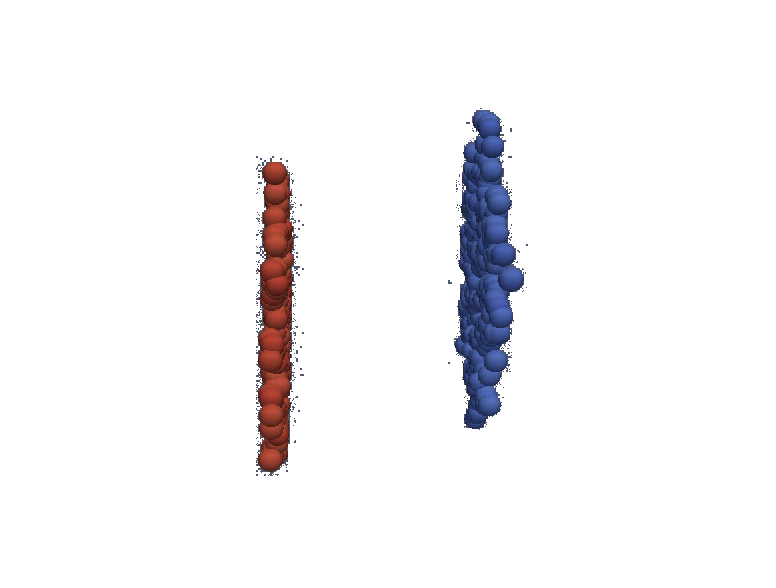
\includegraphics[width=0.2\textwidth]{pics/new1.png} 
	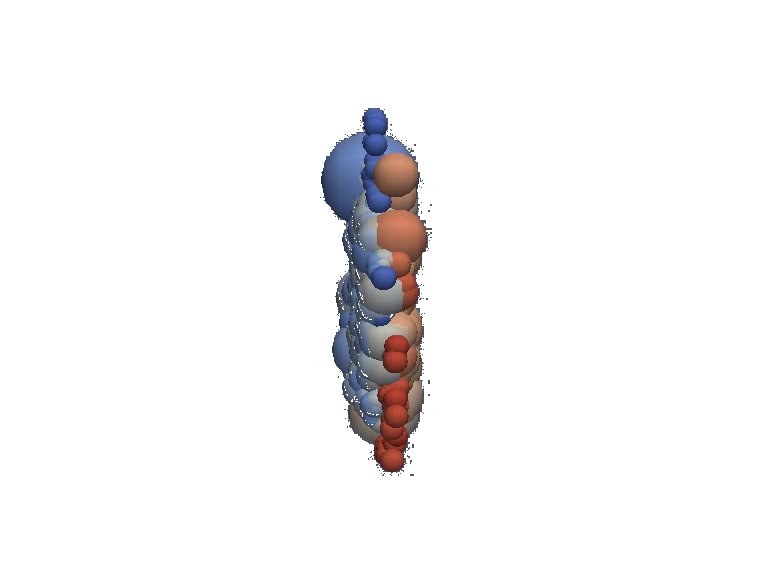
\includegraphics[width=0.2\textwidth]{pics/new50.png} 
	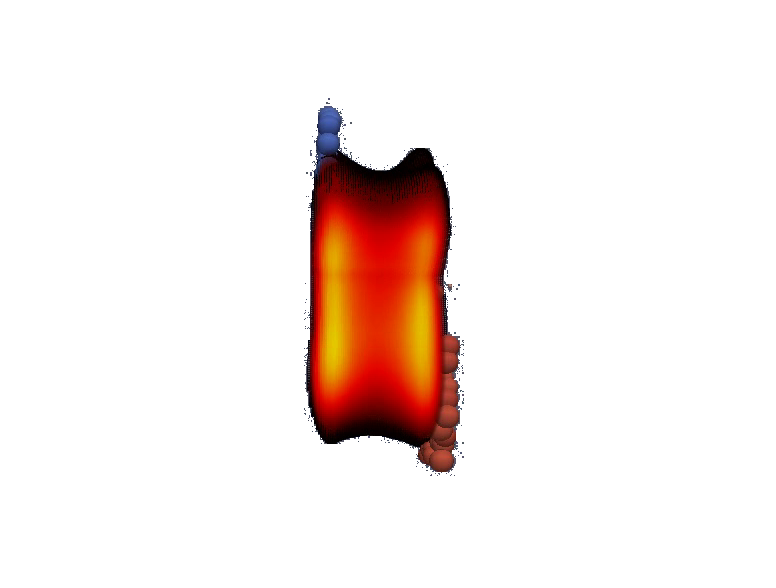
\includegraphics[width=0.2\textwidth]{pics/new100.png}	
	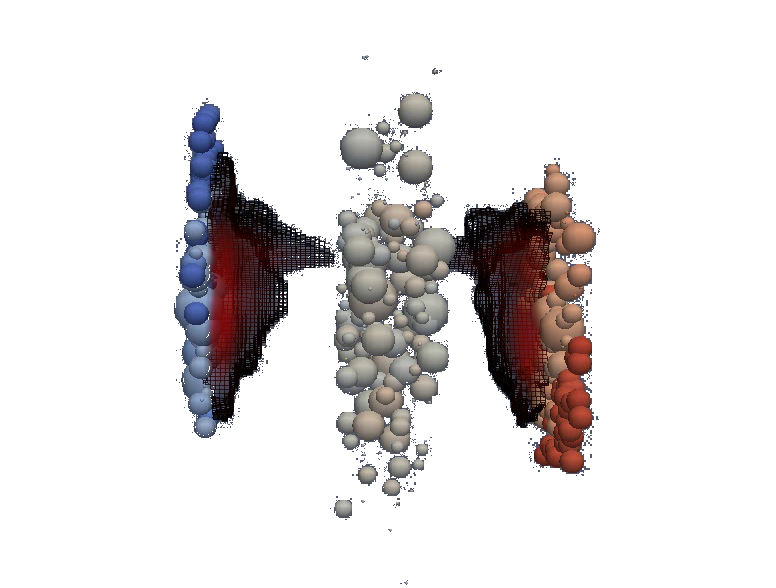
\includegraphics[width=0.2\textwidth]{pics/new230.png}  
	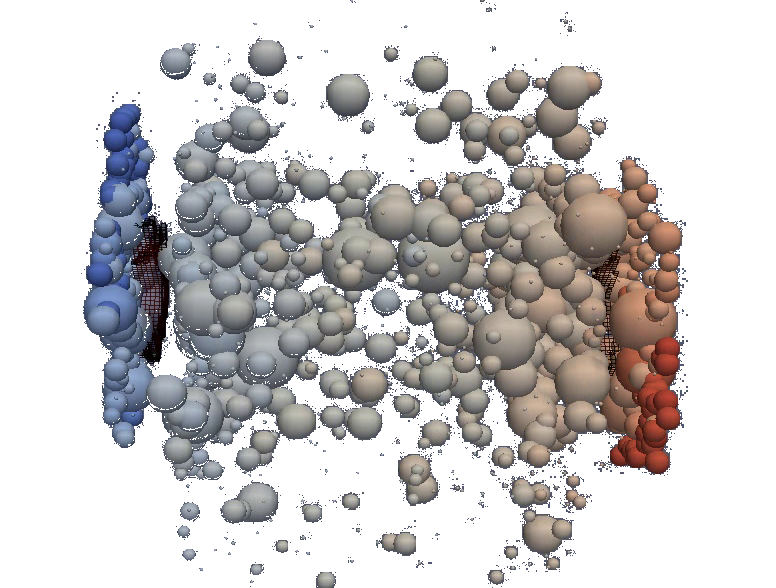
\includegraphics[width=0.2\textwidth]{pics/new300.png}  
	\end{center} 	
  	\end{figure}
  	\begin{center}
  	$\xrightarrow{\makebox[10cm]{Time evolution}}$
  	\end{center}

\begin{itemize}
\item Heavy nuclei are accelerated to nearly the speed of light and collide.
\item Lorentz contraction in beam direction $\rightarrow$ pancake like nuclei.
\item Extremely hot and dense system: $T > 300 \textrm{ MeV} \sim 10^{12} \textrm{ K}$. 
\item Time scale $\sim 10^1 \textrm{ fm/c } (10^{-22} \textrm{ s})$, system size $< 10 \textrm{ fm } (10^{-14}\textrm{ m})$.
\end{itemize}
\end{frame}

\begin{frame}{Nuclear matter in extreme conditions and QGP}
\begin{itemize}
\item Fundamental theory: Quantum Chromodynamics (QCD), describes motion of {\color{red}quarks} and {\color{red}gluons} that carry color charges.
\item Asymptotic freedom at high energy $\rightarrow$ quarks and gluons.
\item Low energy $\rightarrow$ quarks and gluons form bound states (hadrons).
\item Hadrons	$\xrightarrow[\textrm{high } \rho]{\textrm{high } T}$ quark-gluon plasma (QGP)
\end{itemize}

    \begin{figure}
   	\begin{center}
	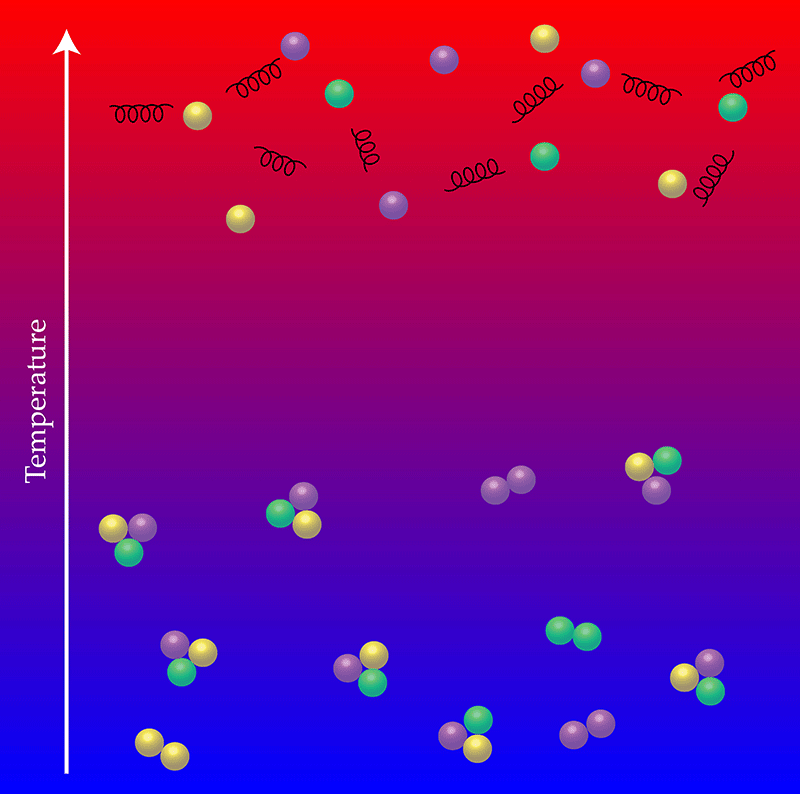
\includegraphics[width=0.35\textwidth]{pics/deconfine.png} 
	
\includegraphics[width=0.05\textwidth]{pics/place_holder.png}
	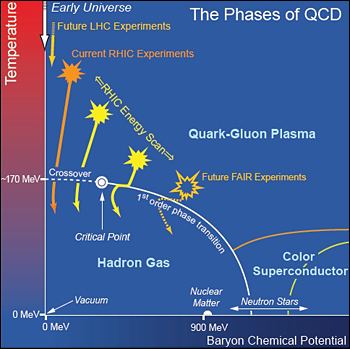
\includegraphics[width=0.35\textwidth]{pics/phase_diagram.jpg} 
	\end{center} 	
  	\end{figure}

\end{frame}

\begin{frame}{QGP at RHIC and LHC}
\begin{itemize}
\item Relativistic Heavy-ion Collider (RHIC) at Brookhaven National Lab (BNL).
	\begin{itemize}
	\item $7.7 - 200 A \textrm{ GeV}$.
	\item Systems, Au+Au, U+U, Cu+Cu, p+Au, d+Au, ${}^3$He+Au ... 
	\end{itemize}
\item Large Hadron Collider (LHC) at the European Organization for Nuclear Research (CERN).
	\begin{itemize}
	\item Increase the energy to TeV regime.
	\item Systems, Pb+Pb ($2.76 A, 5.02 A$ TeV), p+Pb ($5.02 A$ TeV).
	\end{itemize}
\item QGP is produced at both RHIC and LHC.
\end{itemize}
\end{frame}

\begin{frame}{Astonishing properties of QGP: collective phenomena}
\begin{itemize}
\item Fluid behaviour: collective flows. \\Initial spatial anisotropy $\rightarrow$ final momentum anisotropy.
\item Anisotropic flow: azimuthal modulation of momenta distribution.
\begin{eqnarray}
\frac{\mathrm{d}N}{p_T\mathrm{d}p_T\mathrm{d}\phi} \propto 1 + 2{\color{red} v_2} \cos(2(\phi-\Psi_2)) + 2{\color{red}v_3} \cos(3(\phi-\Psi_3)) + ...
\end{eqnarray}
\end{itemize}
\begin{center}
\begin{figure}
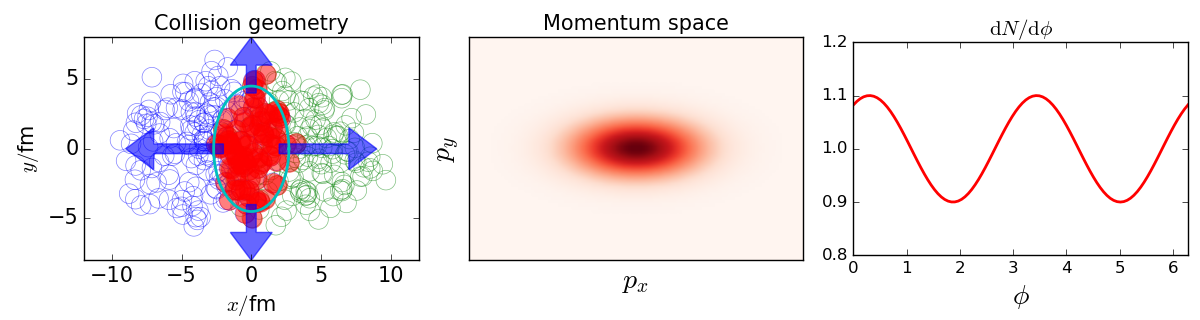
\includegraphics[width=\textwidth]{./pics/nuclei-less.png}
\end{figure}
\end{center}
\end{frame}

\begin{frame}{Astonishing properties of QGP: perfect liquid}
\begin{itemize}
\item Collective behaviour is very well described by relativistic viscous hydrodynamics.
(inputs: $\eta/s$, QCD equation of state.)
\item Viscous effect damps the development of momentum anisotropy.
\item Larger $\eta/s$ $\rightarrow$ smaller final momentum space anisotropy, {\it vice versa}.
\end{itemize}
\begin{center}
\begin{tikzpicture}
  \node[draw=none,fill=blue!0,text=red, rounded corners] (spatial) at (-1,0) {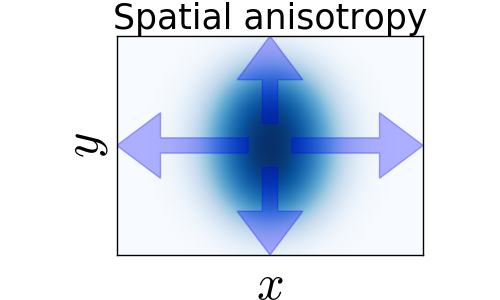
\includegraphics[width=0.3\textwidth]{./pics/almond-0.png}};
  \node[draw=none,fill=blue!0,text=red, rounded corners] (p1) at (-5,0) {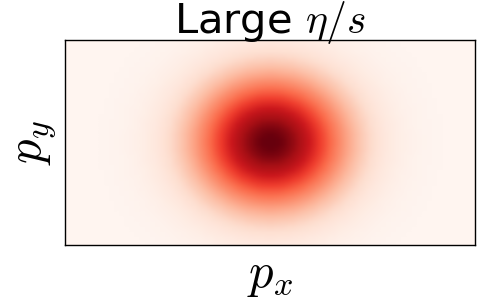
\includegraphics[width=0.3\textwidth]{./pics/almond-p1.png}};
 \node[draw=none,fill=blue!0,text=red, rounded corners] (p2) at (3,0) {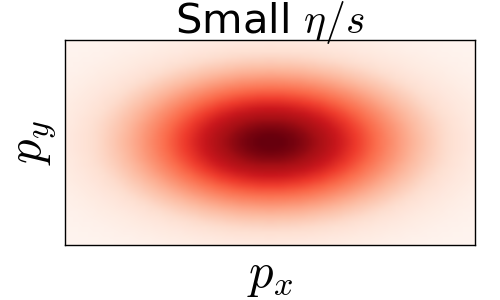
\includegraphics[width=0.3\textwidth]{./pics/almond-p2.png}};
  
  \path[draw=blue!50,solid,line width=1mm,fill=blue!50,
preaction={-triangle 90,thin,draw=blue!50,shorten >=-1mm,fill=blue!50}
] (spatial) to (p1) ;
  \path[draw=blue!50,solid,line width=1mm,fill=blue!50,
preaction={-triangle 90,thin,draw=blue!50,shorten >=-1mm,fill=blue!50}
] (spatial) to (p2) ;
\end{tikzpicture}
\end{center}
\end{frame}

\begin{frame}{Astonishing properties of QGP: perfect liquid}
\begin{itemize}
\item Extract $\eta/s$ by comparing model calculation with experimental data.
\item Extremely low $\eta/s \sim 0.08 - 0.20$, close to quantum lower bound of $\eta/s = \frac{1}{4\pi}$ $\rightarrow$ almost perfect liquid.
\item \color{red}Large uncertainty from initial conditions.
\end{itemize}
\begin{center}
\begin{figure}
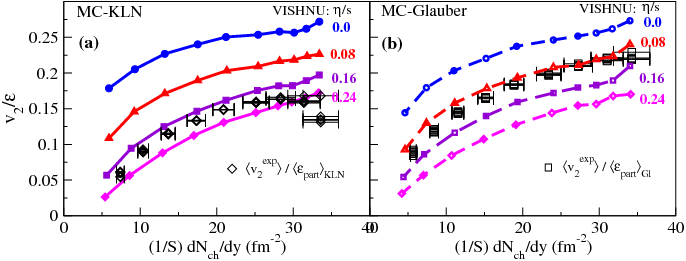
\includegraphics[width=0.56\textwidth]{./pics/song.png}
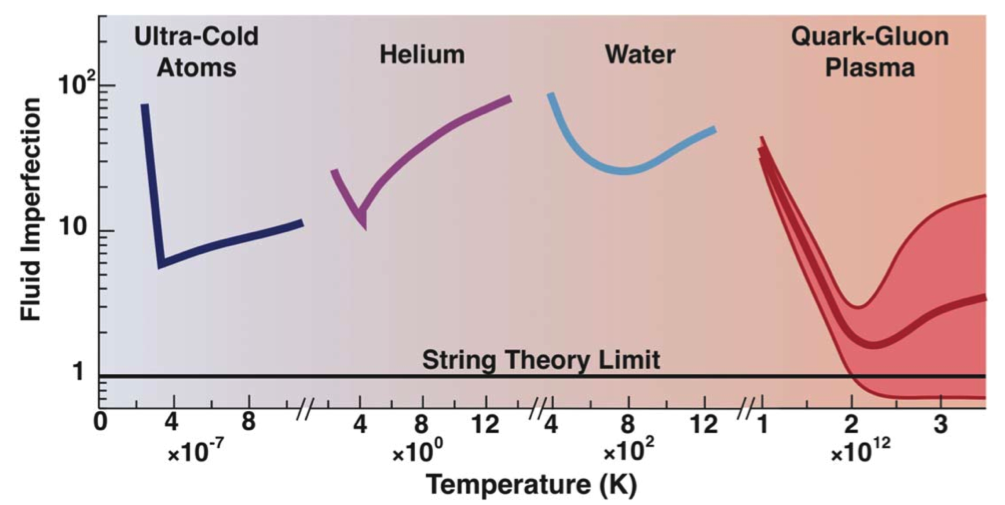
\includegraphics[width=0.44\textwidth]{./pics/eta_s.png}
\end{figure}
\end{center}
\end{frame}

%----------------------------------------------------------------

%------------------------Modelling soft physics------------------
\begin{frame}{Heavy-ion collision modelling}
$\xrightarrow{\makebox[2cm]{Beam axis}}$
    \begin{figure}
   	\begin{center}
	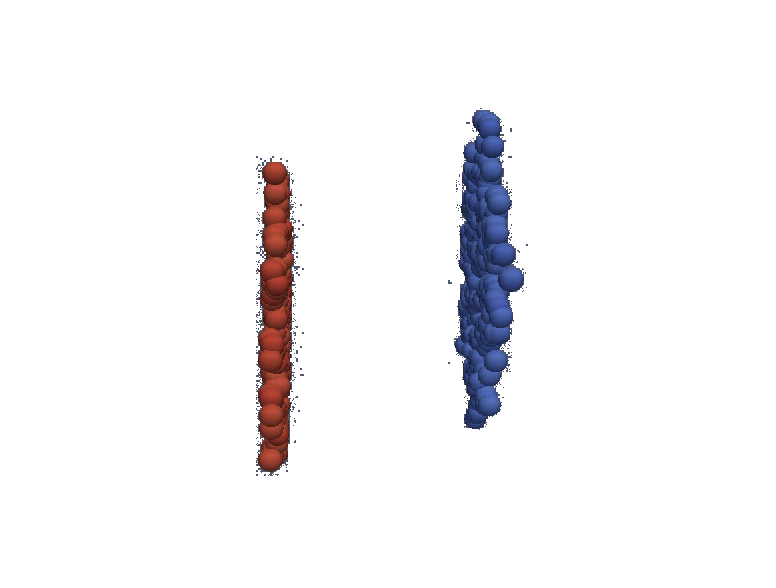
\includegraphics[width=0.2\textwidth]{pics/new1.png} 
	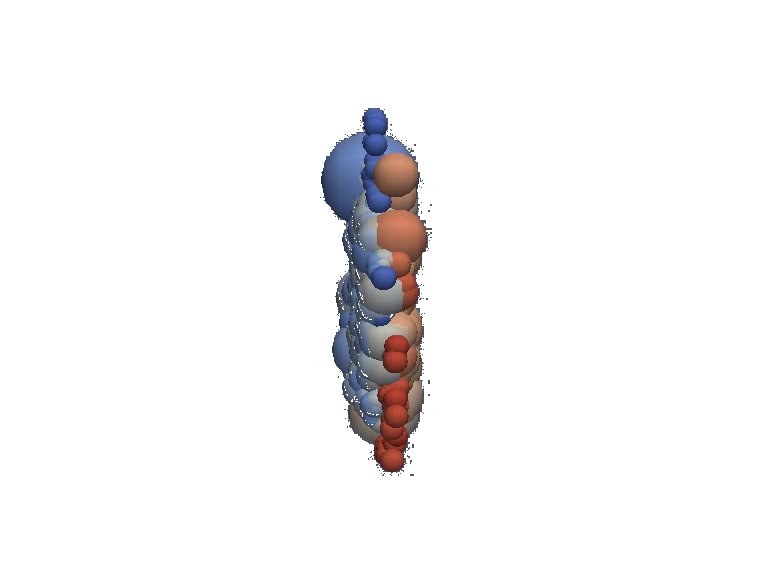
\includegraphics[width=0.2\textwidth]{pics/new50.png} 
	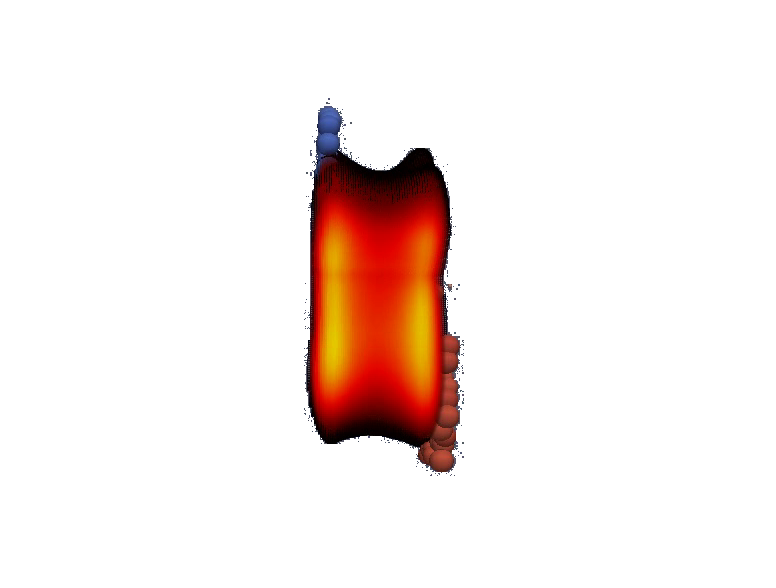
\includegraphics[width=0.2\textwidth]{pics/new100.png}	
	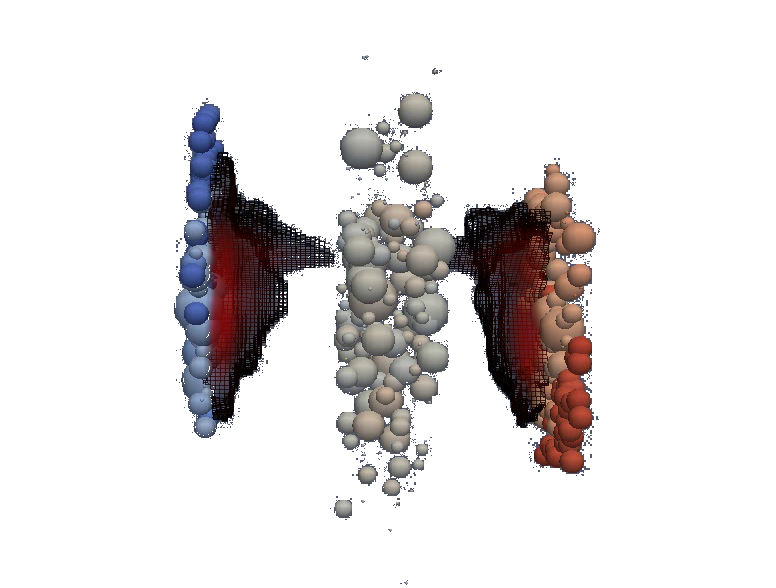
\includegraphics[width=0.2\textwidth]{pics/new230.png}  
	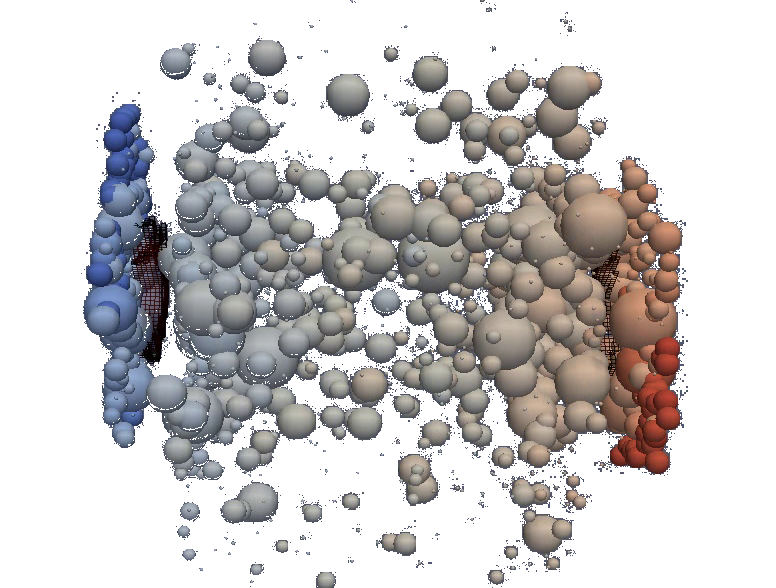
\includegraphics[width=0.2\textwidth]{pics/new300.png}  
	\end{center} 	
  	\end{figure}
  	\begin{center}
  	$\xrightarrow{\makebox[10cm]{Time evolution}}$
  	\end{center}
\begin{center}
\color{blue} Initial states $\rightarrow$  \color{red} QGP \color{blue}  $\rightarrow$ Hadronization $\rightarrow$ Final states interaction $\rightarrow$ Detector
\end{center}
\begin{itemize}
\item Little control of the initial condition; complication from hadronization and final state interaction.
\item Need a modelling of systems' full time evolution and extract QGP properties by model-to-data comparison.
\end{itemize}
\end{frame}

\begin{frame}{Initial state ($< 1 \textrm{ fm/c}$)}
\begin{columns}[onlytextwidth]
  \begin{column}{0.25\textwidth}
  \begin{figure}
   	\begin{center}
	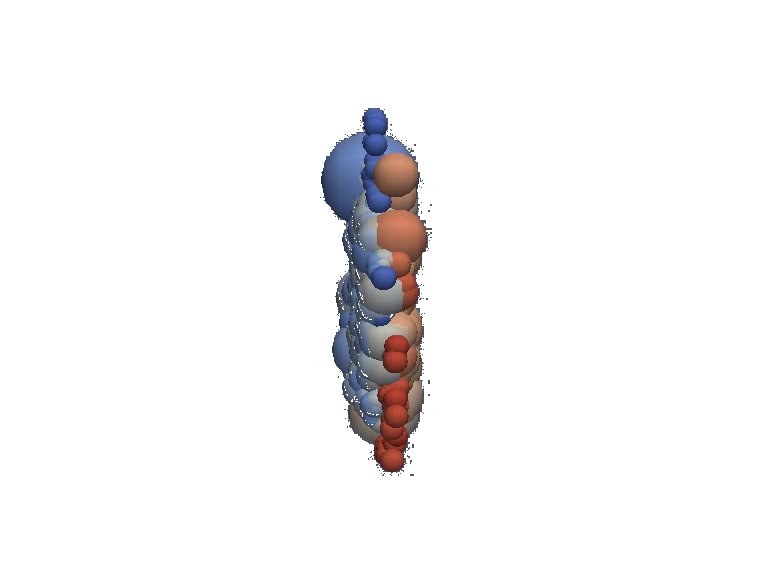
\includegraphics[width=\textwidth]{pics/new50.png} 
	\end{center} 	
  	\end{figure} 
  \end{column}
  \begin{column}{0.75\textwidth}
  	\begin{itemize}
	\item Initially far from thermal equilibrium.
	\item Studies suggests fast thermalization proscess towards local thermal equilibrium ($< 1 \textrm{ fm/c}$).
	\item Mechanism not very well understood.
\end{itemize}
  \end{column}
\end{columns}  


\tikzstyle{block} = [rectangle, draw, fill=blue!20, 
    text width=14em, rounded corners, minimum height=6em]
\begin{center}
\begin{tikzpicture}
  \node[block] (model1) at (-3, 0) {{\color{red} Dynamical models}: include pre-equilibrium dynamics; then match to local thermal equilibrium initial energy density.};
  \node[block] (model2) at (3, 0) {{\color{red} Parametric models}: phenonmenolgical model that provide entropy / energy density at later time assuming local thermal equilibrium.};
\end{tikzpicture}
\end{center}


\end{frame}

\begin{frame}{Hydrodynamics $\rightarrow$ particlization $\rightarrow$ hadronic scattering}

\begin{columns}[onlytextwidth]
  \begin{column}{0.2\textwidth}
    \begin{figure}
   	\begin{center}
   	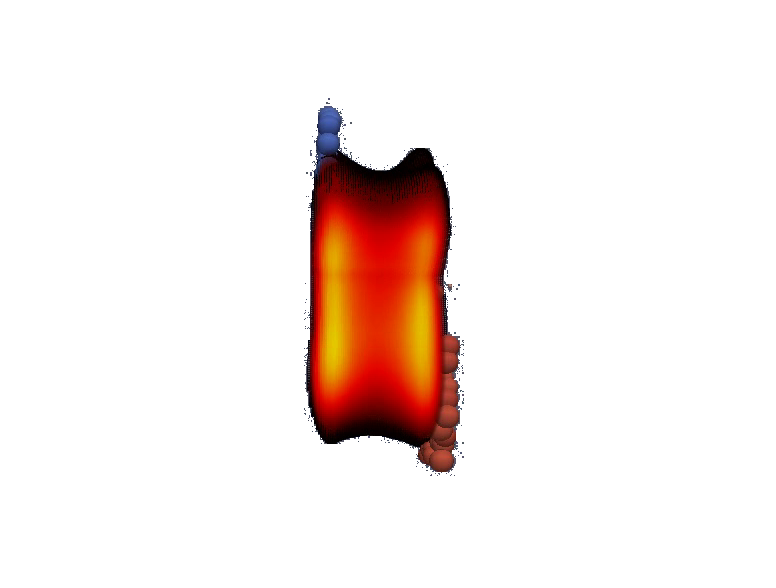
\includegraphics[width=\textwidth]{pics/new100.png}
	\end{center} 	
  	\end{figure}
  \end{column}
  \begin{column}{0.8\textwidth}
  \begin{itemize}
  	\item System closes to local thermal equilibrium.
  	\item Energy momentum and charge conservation,
  	\begin{eqnarray}
  	{\partial}_\nu T^{\mu\nu} = 0, {\partial}_\nu N^{\nu} = 0.
  	\end{eqnarray}
  	\item Closed by QCD equation of state $\epsilon = \epsilon(p)$.
  \end{itemize}
  \end{column}
\end{columns}
\begin{center}
\kern-0.5em
\rule{11cm}{0.5pt}
\end{center}
\kern-2em
\begin{columns}[onlytextwidth]
  \begin{column}{0.85\textwidth}
  \begin{itemize}
  	\item The expanding system becomes dilute and hydrodynamics ceases to apply. 
  	\item Particlize energy density to hadrons.
  \end{itemize}
  \end{column}
  \begin{column}{0.2\textwidth}
    \begin{figure}
   	\begin{center}
   	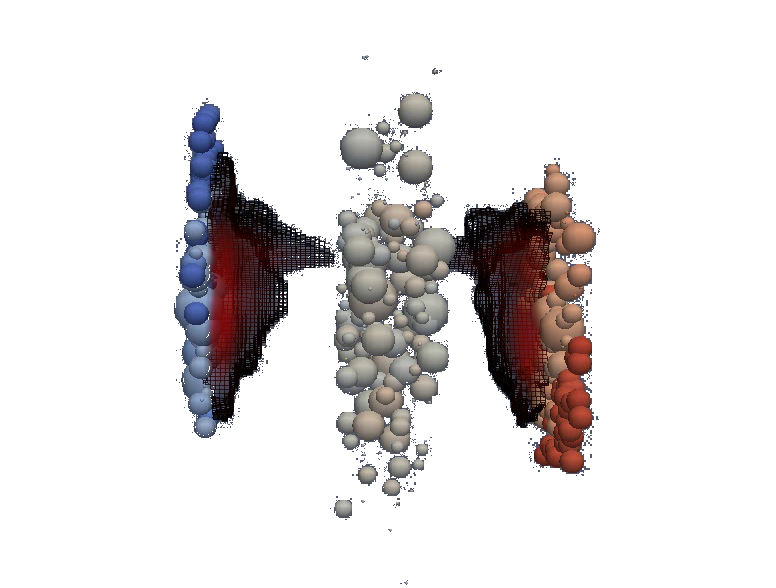
\includegraphics[width=\textwidth]{pics/new230.png}
	\end{center} 	
  	\end{figure}
  \end{column}
\end{columns}
\kern-1em
\begin{center}
\rule{11cm}{0.5pt}
\end{center}
\kern-2em
\begin{columns}
 \begin{column}{0.15\textwidth}
    \begin{figure}
   	\begin{center}
   	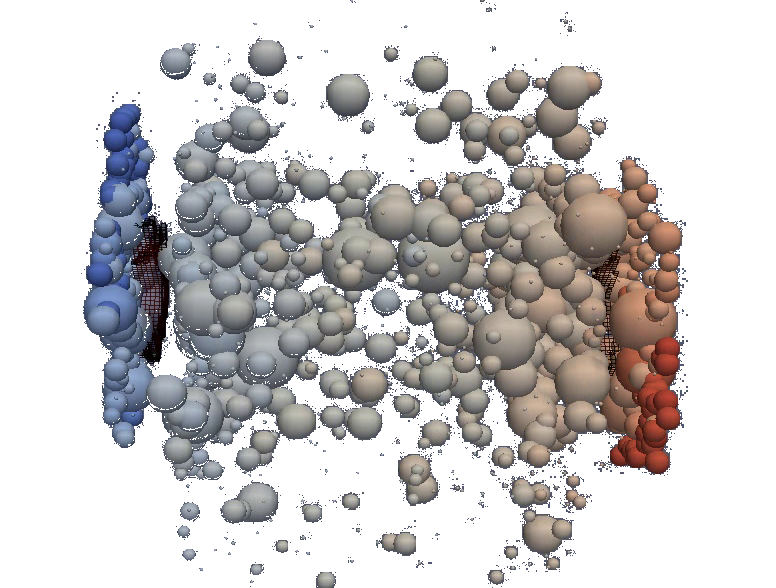
\includegraphics[width=\textwidth]{pics/new300.png}
	\end{center} 	
  	\end{figure}
  \end{column}
  \begin{column}{0.85\textwidth}
  \begin{itemize}
  	\item System is still dense to allow hadronic scattering.
	\item Solving Boltzmann transport equation of hadrons.
  \end{itemize}
  \end{column}
\end{columns}

\end{frame}

%----------------------------------------------------------------

%-----------------------3d IC------------------------------------
\section{TRENTo initial condition model}
\begin{frame}{Kinematics for fast expansion system}
Define proper time $(\tau)$ and space-time rapidity $(\eta_s)$,
\begin{eqnarray}
\tau = \sqrt{t^2 - z^2}, \eta_s = \frac{1}{2}\ln\frac{t+z}{t-z}. 
\end{eqnarray}
Final particle momenta, define rapidity $(y)$ or pseudo-rapidity $(\eta)$,
\begin{eqnarray}
 y = \frac{1}{2}\ln\frac{E+p_z}{E-p_z}, \eta &=& \frac{1}{2}\ln\frac{|\mathbf{p}|+p_z}{|\mathbf{p}|-p_z} = -\ln\left(\tan\frac{\theta}{2}\right). 
\end{eqnarray}
\begin{center}
\begin{figure}
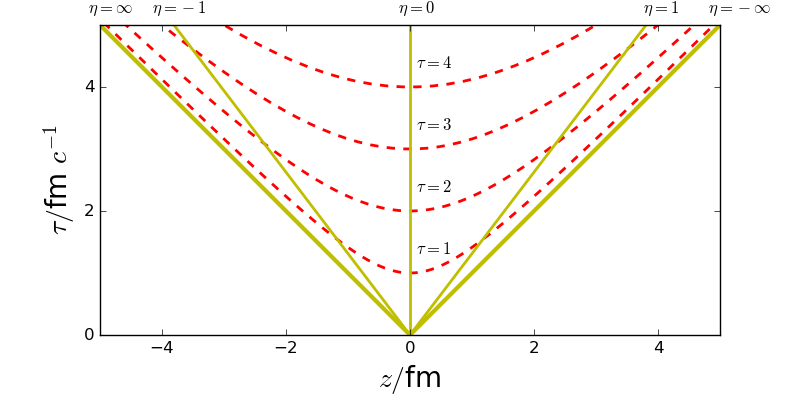
\includegraphics[width=0.7\textwidth]{./pics/curv.png}
\end{figure}
\end{center}
\end{frame}

\begin{frame}{Boost-invariance approximation}
\begin{itemize}
\item Boost-invariance approximation: system is independent of $\eta_s$ or invariant by a shift in rapidity.
\item Reduces 3+1 d hydrodynamics to 2+1 d, requires a 2d initial condition.
\item A good approximation for large, symmetric collisions (Au+Au, Pb+Pb) within $-2 < \eta < 2$.
\end{itemize}
\begin{center}
\begin{figure}
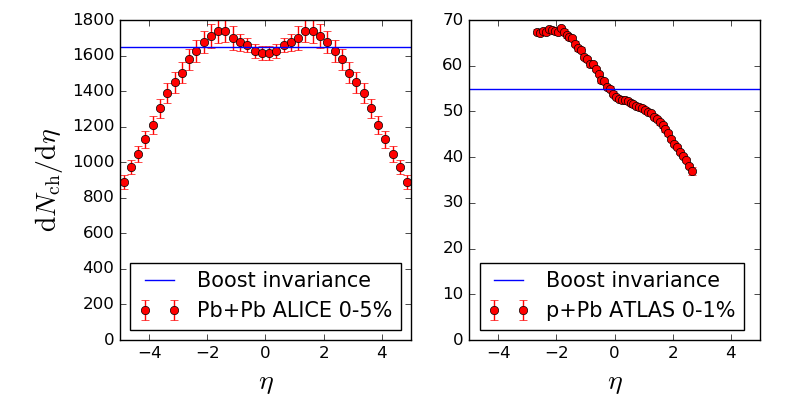
\includegraphics[width=0.7\textwidth]{./pics/bi.png}
\end{figure}
\end{center}
\end{frame}

\begin{frame}{General structure of TRENTo IC}
TRENTo (PRC.92.011901)\\
An effective model of initial condition assuming boost invariance and provided initial 2d entropy density $s(x_\perp)$ at mid-rapidity ($\eta_s = 0$).
\\
TRENTo IC is developed in three layers:
\begin{itemize}
\item Glauber calculation of nucleon-nucleon collision.
\item Determine the density of participant matter.
\item Map participant density to mid-rapidity entropy deposition.
\end{itemize}
\end{frame}

\begin{frame}{Glauber calculation of nucleon-nucleon collision}
\begin{itemize}
\item Collision probability with impact parameter $b$,
\begin{eqnarray}\label{dsigma_db}
		P_{\textrm{coll}}(b) &=& \frac{\mathrm{d}\sigma_{NN}}{2\pi b \mathrm{d}b} = 1 - \exp\left(-\alpha T_{pp} (b)\right). \\
		T_{pp} &=& \int \mathrm{d}x_\perp \rho\left(x_\perp + \frac{b}{2}\right) \rho\left(x_\perp - \frac{b}{2}\right).
\end{eqnarray}
\end{itemize}
\begin{columns}[onlytextwidth]
  \begin{column}{0.4\textwidth}
    \begin{figure}
	\begin{center}
	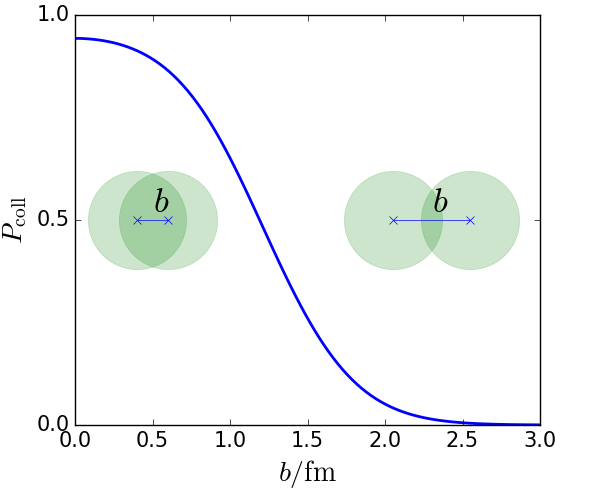
\includegraphics[width = \textwidth]{./pics/Pcoll.png}
	\end{center}
	\end{figure}
  \end{column}
  \begin{column}{0.6\textwidth}
  \begin{itemize}
  	\item Parameter $\alpha$ is tuned to match experimental cross-section $\sigma_{pp, \textrm{inel}}(\sqrt{s})$.
  	\item $T_{pp}(b)$: overlapping between two nucleons' density.
  	\item Nucleon density modelled by normal distribution.
  \end{itemize}
  \end{column}
\end{columns}
\end{frame}

\begin{frame}{Calculating participant density}
\begin{columns}
\begin{column}{0.7\textwidth}
\begin{itemize}
\item Nucleons are sampled from averaged nucleon distribution inside a nuclei.
\item Check each pair of target/projectile nucleons for collision.
Nucleons collides at least once are called participants.
\end{itemize}
\end{column}
\begin{column}{0.3\textwidth}
\begin{figure}
\begin{center}
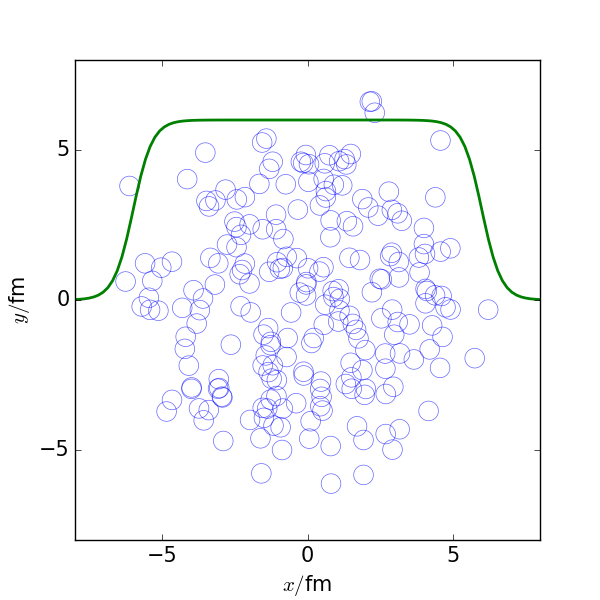
\includegraphics[width = \textwidth]{./pics/WS2.png}
\end{center}
\end{figure}
\end{column}
\end{columns}

\begin{columns}
\begin{column}{\textwidth}
\begin{itemize}
\item Participant density of nuclei $A$ and $B$,
\begin{eqnarray}
	T_{A,B}(x_\perp) = \sum_{i \in \textrm{Part} A,B} \gamma_i \rho(x_\perp- x_i), \gamma_i &\sim& \Gamma(k, k)
\end{eqnarray}
\item Additional $\Gamma$ fluctuation to correctly reproduce experimental $pp$ multiplicity fluctuation.
\end{itemize}
\end{column}
\begin{column}{0.0\textwidth}
\end{column}
\end{columns}
\end{frame}

\begin{frame}{2d entropy deposition ansatz at mid-rapidity}
\begin{itemize}
\item Mapping participant density to mid-rapidity entropy deposition,
	\begin{equation}
		\mathrm{d}S/\mathrm{d}\eta_s(x_\perp) \propto T_R(T_A, T_B; p) = \left(\left(T_A^p(x_\perp) + T_B^p(x_\perp)\right)/2\right)^{\frac{1}{p}}.
	\end{equation}
\item Mimic a variety of models at mid-rapidity (J. S. Moreland):
\begin{center}
\begin{tabular}{cccc}
\hline 
p $\sim$ & -0.67 & 0.0  & 1.0 \\ 
\hline 
model  & KLN   & EKRT & Glauber (participant scaling) \\ 
\hline 
\end{tabular} 
\end{center}
\item A model-to-data comparison (J. E. Bernhard) suggests $p \approx 0$.
\end{itemize}
\begin{center}
\begin{figure}
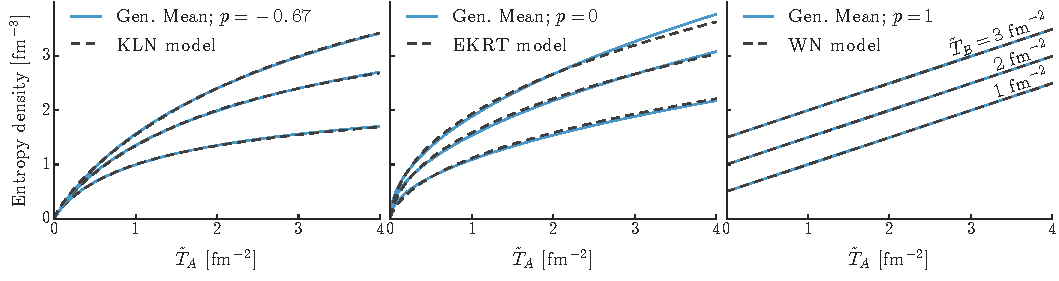
\includegraphics[width=\textwidth]{./pics/cgc_compare.pdf}
\end{figure}
\end{center}
\end{frame}

\section{Rapidity dependent TRENTo initial condition model}
\begin{frame}{3d IC motivation: QGP in small systems?}
\begin{itemize}
\item QGP was not expected in small system  d+Au, p+Pb
$\rightarrow$ but similar collective phenomena observed.
\item QGP in small systems? Is hydrodynamics applicable?
\item Boost-invariance is not a good approximation in asymmetry collision (d+Au, p+Pb). A rapidity dependent IC is demanding.
\end{itemize}
\begin{center}
\begin{figure}
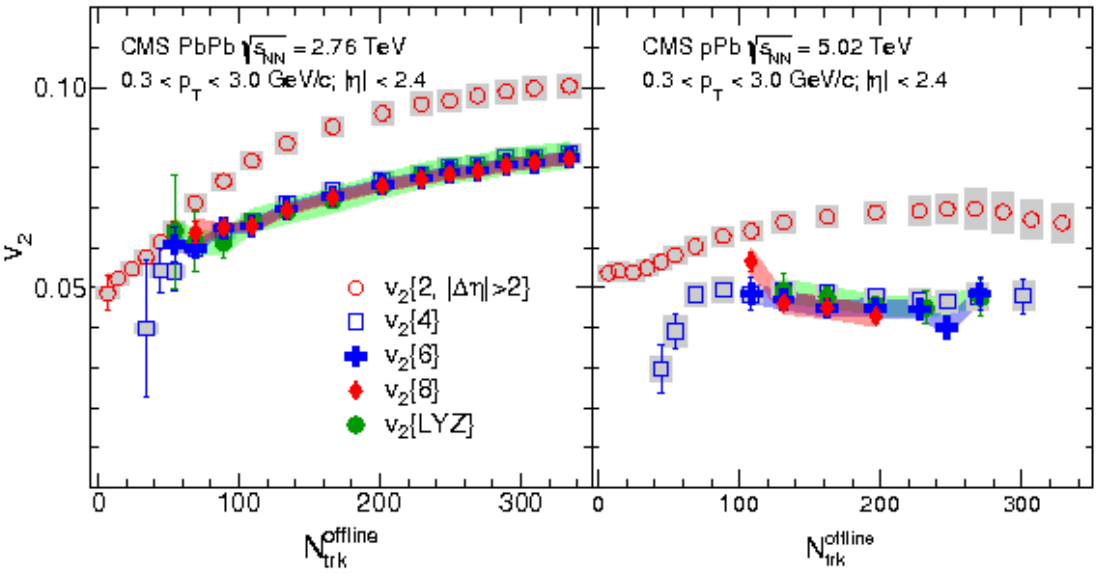
\includegraphics[width=0.6\textwidth]{./pics/small.png}
\end{figure}
\end{center}
\end{frame}

\begin{frame}{3d IC motivation: effect of longitudinal fluctuation}
\begin{itemize}
\item Even in large system, boost-invariance only works for event-averaged distributions.
\item Single events contain longitudinal fluctuations.
\item Study fluctuation effects on the extraction of QGP properties.
\end{itemize}
\end{frame}

\begin{frame}{3d IC motivation: rapidity dependent observables}
\begin{itemize}
\item $\eta$ dependent observables could be sensitive to QGP properties and IC.
\item E.g. pseudo-rapidity dependence of flows is sensitive to temperature dependence of $\eta/s$ (Gabriel Denicol, arXiv:1512.08231).
\end{itemize}
\begin{center}
\begin{figure}
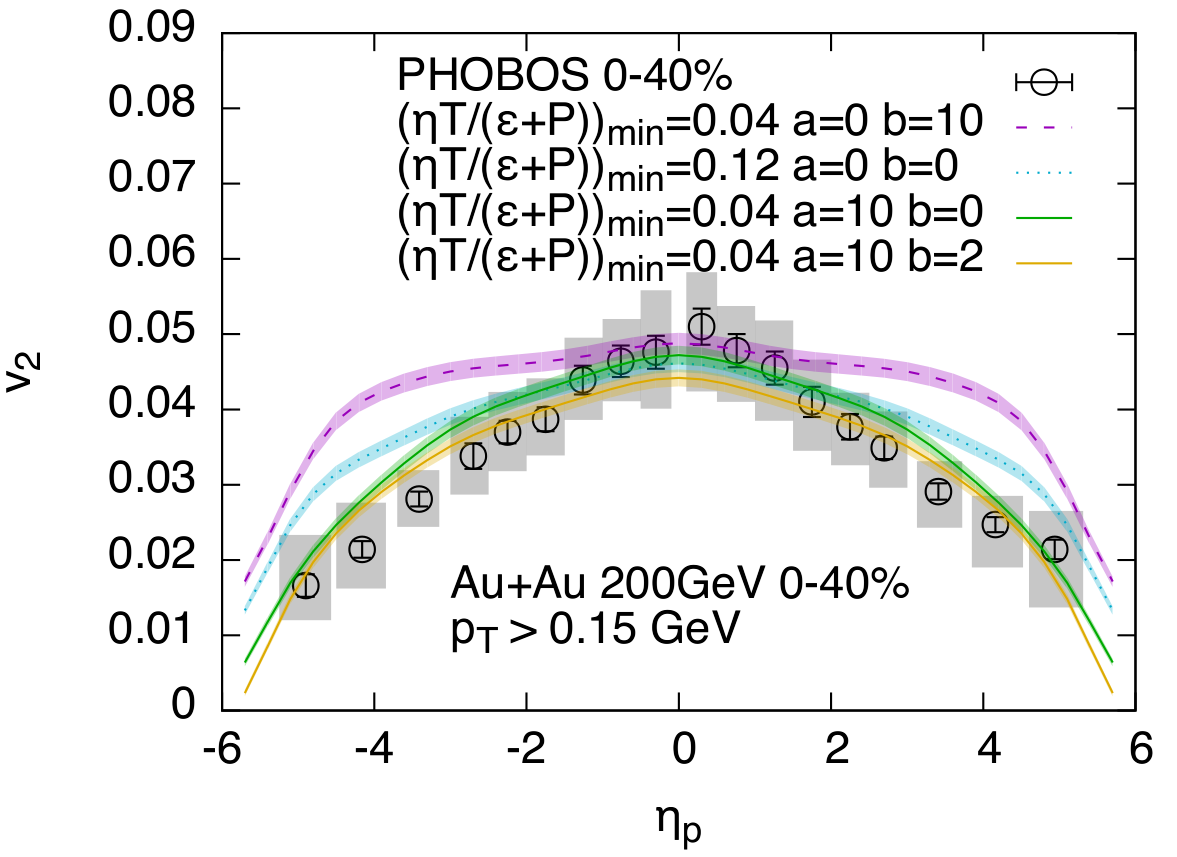
\includegraphics[width=0.575\textwidth]{./pics/Bjorn-v2-eta.png}
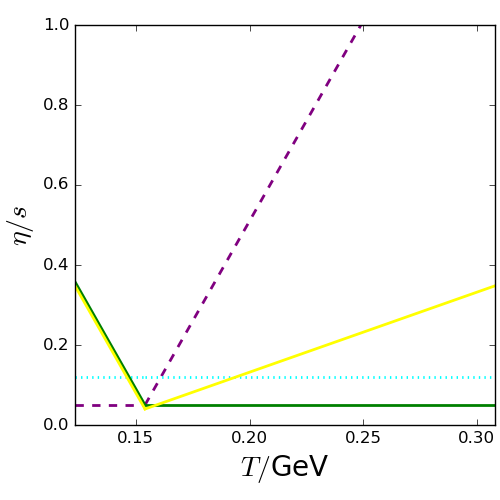
\includegraphics[width=0.425\textwidth]{./pics/etaS-Bjorn.png}
\end{figure}
\end{center}
\end{frame}

\begin{frame}{Formula: from 2d to 3d}
In TRENTo 2d:
\begin{itemize}
\item Glauber calculation of nucleon-nucleon collision.
\item Determine the density of participant matter.
\item Map participant density to mid-rapidity entropy deposition.
\end{itemize}
Toward TRENTo 3d:
\begin{itemize}
\item \color{red} Determine local rapidity profile from participant density.
\begin{eqnarray}
	T_A(x_\perp), T_B(x_\perp) &\rightarrow& T_R(x_\perp, \eta)
\end{eqnarray}
\item Simple and flexible $\rightarrow$ suitable for parametrize a variety of models.
\item Preserve TRENTo 2d calculation at mid-rapidity.
\end{itemize}
\end{frame}

\begin{frame}{Formula: from 2d to 3d}
\begin{itemize}
\item Factorize $\perp$ and $\parallel$ to reproduce mid-rapidity TRENTo result.
\begin{eqnarray}
	T_R(x_\perp, \eta) = T_R(x_\perp)f(x_\perp, \eta), f(x_\perp, 0) = 1.
\end{eqnarray}
\item For flexibility, use no explicit form of $f$. $f((x_\perp), \eta)$ characterized by its cumulants,

\begin{center}
\begin{tabular}{c|c|c|c}
\hline
	mean	 	&	std   	&	skewness		&	kurtosis		\\
\hline
	$\mu(x_\perp)$	& $\sigma(x_\perp)$ & $\gamma(x_\perp)$ & $\kappa(x_\perp)$	\\
\hline
\end{tabular}
\end{center}

\item Reconstruct $ f(\eta) $ by $\mathscr{F}^{-1}$ cumulant generating function:
\begin{eqnarray}\label{naive_fourier}
	 \mathscr{F}^{-1}\exp\left(i \mu k - \frac{\sigma^2}{2}k^2 + i \gamma k^3 - \kappa k^4 \right)
\end{eqnarray}
\end{itemize}
\end{frame}

\begin{frame}{Encoding models}
\begin{itemize}
\item Existing parametrizations (Piotr Bozek, arXiv:1002.4999),\\
Shifted: $f(\eta_s) \rightarrow f(\eta_s - \mu)$;  tilted: $f(\eta_s) \rightarrow f(\eta_s) \left(1 + \gamma\eta_s/y_{\textrm{beam}}\right)$.
\item $\mu$ and $\gamma$ measures the local asymmetry of participant density.
\end{itemize}
\begin{center} 
\begin{figure}
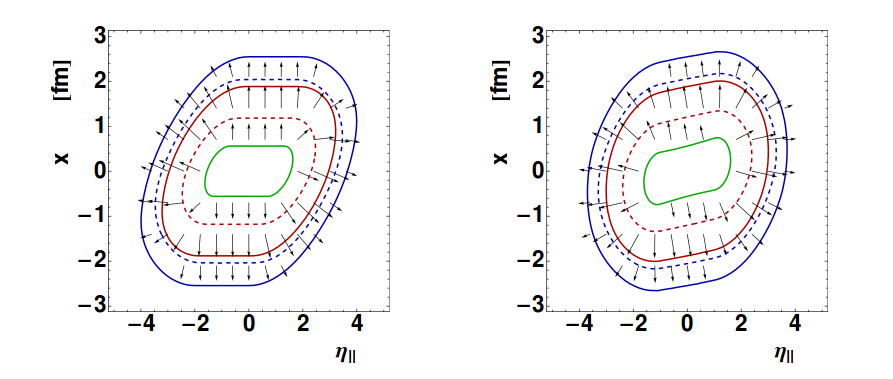
\includegraphics[width=0.6\textwidth]{pics/Pitor.png} 
\end{figure}
\begin{tabular}{c|c|c|c|c}
\hline
--	&	$\mu$	& $\sigma$ & $\gamma$ & $\kappa$	\\
\hline
shifted & $\frac{1}{2}\log\left(\frac{T_A}{T_B}\right)$ & const. & $0$	& const. \\
tilted & $0$ & const. & $\frac{T_A-T_B}{T_A+T_B}, T_A - T_B, etc$	& const.\\
general & $\frac{a}{2}\log\left(\frac{T_A}{T_B}\right)$ & $b$ & $c(T_A - T_B)$ & $d$ \\
\hline
\end{tabular}
\end{center}
\end{frame}

\begin{frame}{Sample 3d events}
\begin{itemize}
\item Strong local longitudinal fluctuation in Pb+Pb collisions.
\item Asymmetric rapidity profile for pPb collisions.
\end{itemize}
\begin{figure}
\begin{center}
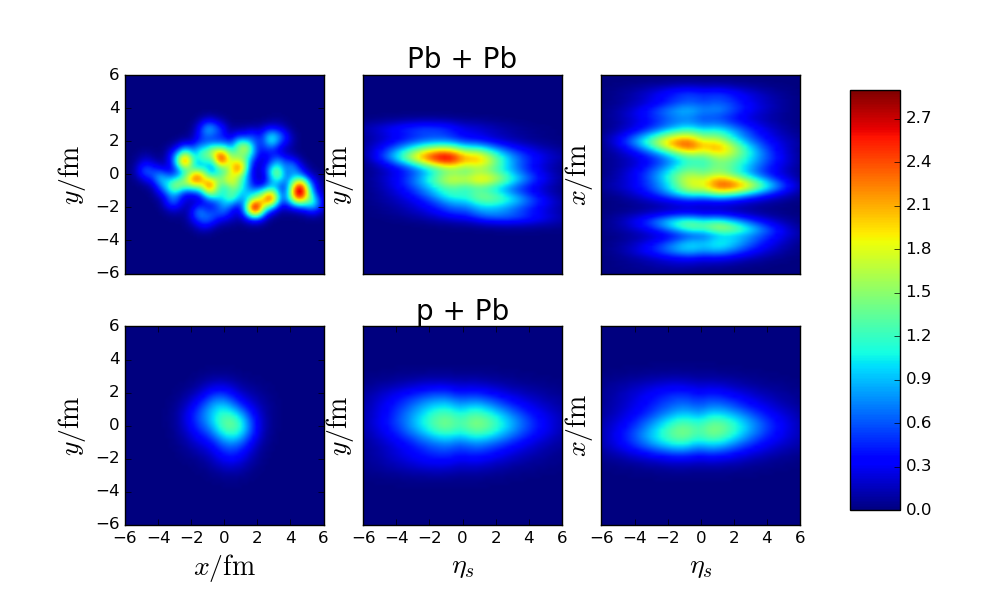
\includegraphics[width = 0.8\textwidth]{./pics/3d-example.png}
\end{center}
\end{figure}
\end{frame}

%----------------------------------------------------------------

%-----------------------Model-to-data Comparison-----------------
\section{Inference of IC parameters from model-to-data comparison}
\begin{frame}{IC directly against experiment}
\begin{itemize}
\item Time evolution (3+1 D hydrodynamics) is computationally expensive.
\item First compare 3d initial condition model with observables not sensitive to time-evolution $\rightarrow$ crude inference of IC parameters.
\item Charged particle pseudo-rapidity distribution works well,
	\begin{eqnarray}
		\mathrm{d}N_{\textrm{ch}}/\mathrm{d}\eta \propto \mathrm{d}s/\mathrm{d}\eta_s
	\end{eqnarray}
	Can be checked later.
\end{itemize}
Tools: model-to-data comparison by Bayesian analysis.
\end{frame}

\begin{frame}{Parameter design: Latin-hypercube sampling}
\begin{itemize}
\item 3d initial condition introduces about 4-5 more parameters. A high dimensional parameter space:
\begin{center}
\begin{tabular}{ccccccc}
\hline
fluctuation & norm  & 	mean	 	&	std   	&	skewness		&	kurtosis	 & Jacobi	\\
\hline
$k$ & $N$ & $a$ & $b$ & $c$ & $d$ & $J$ \\
$[1,4]$ & $[8,12]$ & $[0,2]$ & $[2,4]$ & $[0, 0.5]$ & $[0.2, 0.8]$ & $[0.6, 0.8]$\\
\hline
\end{tabular}
\end{center}
\item Latin-hypercube sampling: \\Monte-Carlo sampling of parameter points $x_i$ from $[0, 1]^d$.
\item Avoid over populated / sparse regions, $N_{\textrm{samples}} \propto d$.
\item Compute model output $y_i$ on design parameter sets $x_i$,
\begin{eqnarray}
	x_i \xrightarrow{Model} y_i.
\end{eqnarray}
\end{itemize}
\end{frame}

\begin{frame}{Gaussian process emulator: interpolate over design point}
\begin{itemize}
\item Gaussian process: a set of random variables, any finite number of which have a joint Gaussian distribution.
\item Draw random functions specified by the mean and covariance,
\begin{eqnarray}
\Sigma(x_1, x_2) = \sigma^2 \exp\left(-\frac{\left(x_1 - x_2\right)^2}{2l^2}\right)
\end{eqnarray}
\end{itemize}
\begin{center}
\begin{figure}
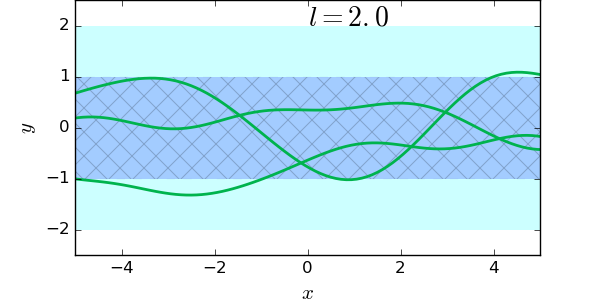
\includegraphics[width = 0.5\textwidth]{./pics/GP-1.png}
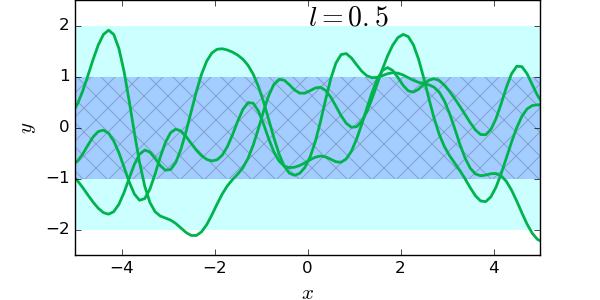
\includegraphics[width = 0.5\textwidth]{./pics/GP-11.png}
\end{figure}
\end{center}
\end{frame}

\begin{frame}{Gaussian process emulators: interpolate over design point}
\begin{itemize}
\item Gaussian process emulator: a Gaussian process conditioned with input parameter sets $x_i$ and model outputs $y_i$.
\item Make inference of model output with arbitrary parameter sets with likelihood.
\item Gaussian process emulator is a fast surrogate for computationally intense model.
\end{itemize}
\begin{center}
\begin{figure}
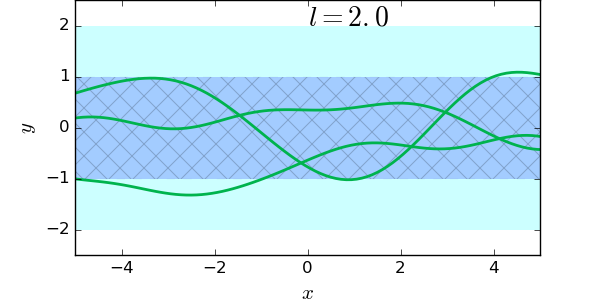
\includegraphics[width = 0.5\textwidth]{./pics/GP-1.png}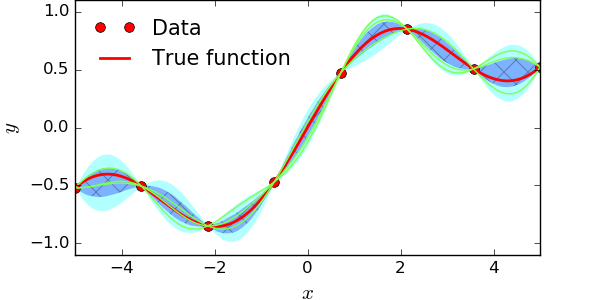
\includegraphics[width = 0.5\textwidth]{./pics/GP-2.png}
\end{figure}
\end{center}
\end{frame}

\begin{frame}{Model-to-data comparison flow chart}
\begin{center}
\begin{figure}
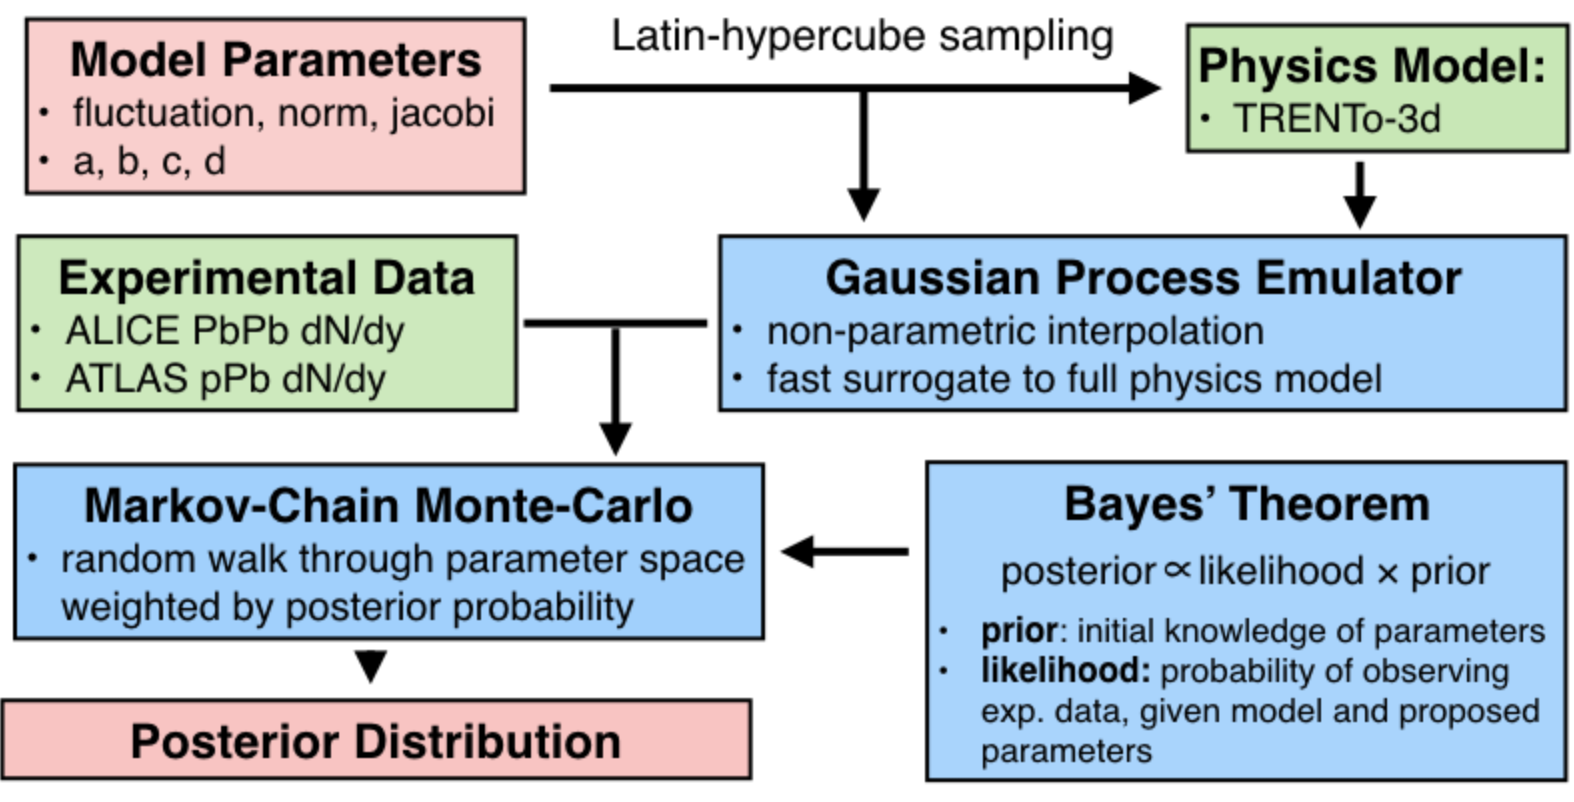
\includegraphics[width=\textwidth]{./pics/flow-chart.png}
\end{figure}
\end{center}
\end{frame}

%----------------------------------------------------------------

%-----------------------Results-----------------
\section{Results}
\begin{frame}{Prior / posterior of model output}
\begin{itemize}
\item $\mathrm{d}N/\mathrm{d}\eta$ from parameters draw from priori / posterior distributions, comparing to Pb+Pb data @ $2.76A$ TeV. 
\item The model can very well describes Pb+Pb data of different multiplicities.
\end{itemize}
\begin{figure}
\begin{center}
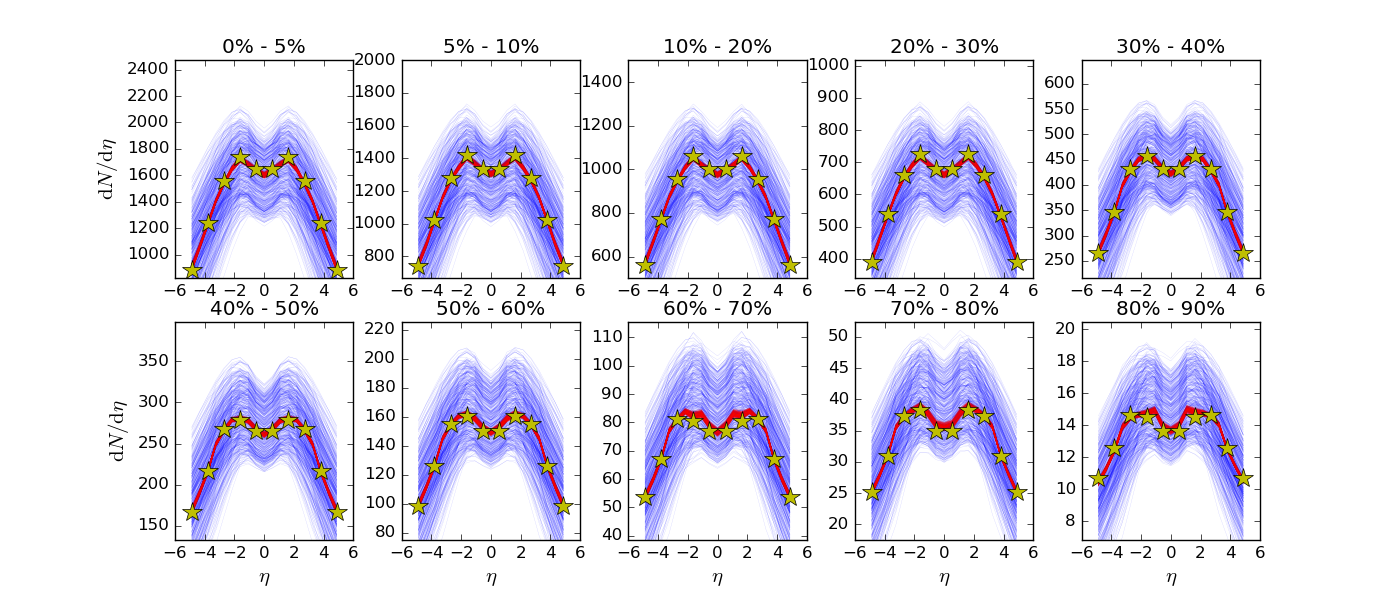
\includegraphics[width = \textwidth]{./pics/pri-post-PbPb.png}
\end{center}
\end{figure}
\end{frame}

\begin{frame}{Prior / posterior of model output}
\begin{itemize}
\item $\mathrm{d}N/\mathrm{d}\eta$ from parameters draw from priori / posterior distributions, comparing to p+Pb data @ $5.02A$ TeV. 
\item The model reproduces the asymmetry distribution of different multiplicities in small system.
\end{itemize}
\begin{figure}
\begin{center}
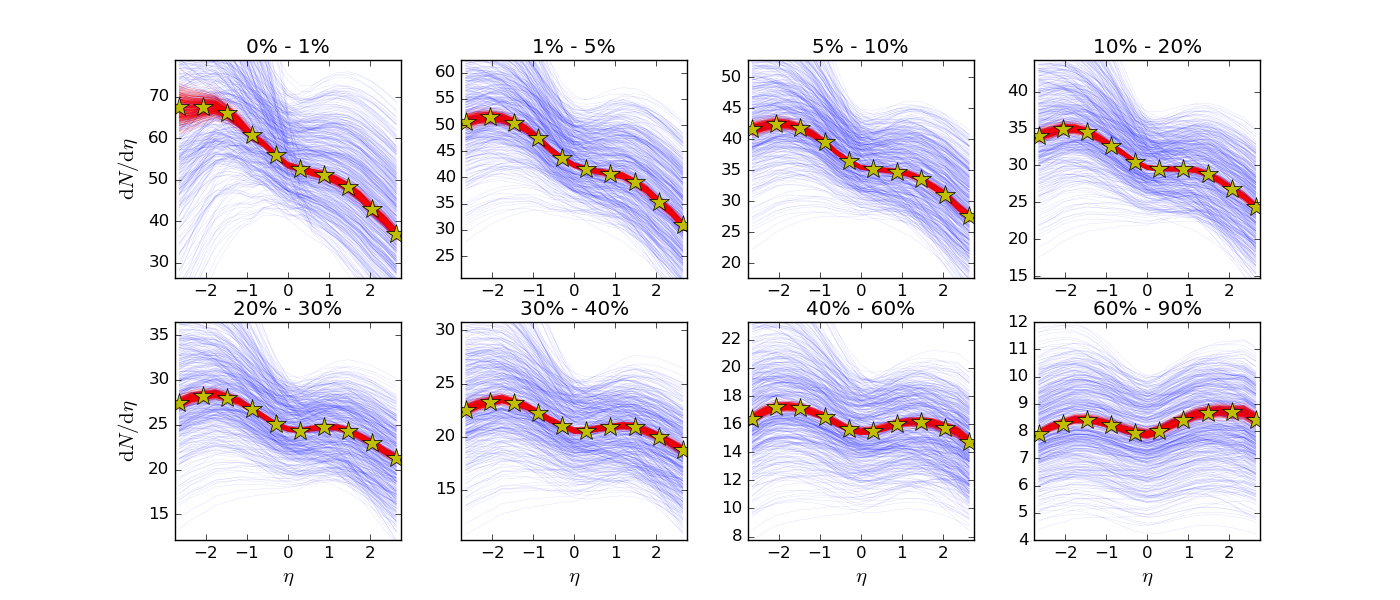
\includegraphics[width = \textwidth]{./pics/pri-post-pPb.png}
\end{center}
\end{figure}
\end{frame}

\begin{frame}{Marginalized posterior distribution of model parameters}
\begin{columns}
\begin{column}{0.6\textwidth}
\begin{figure}
\begin{center}
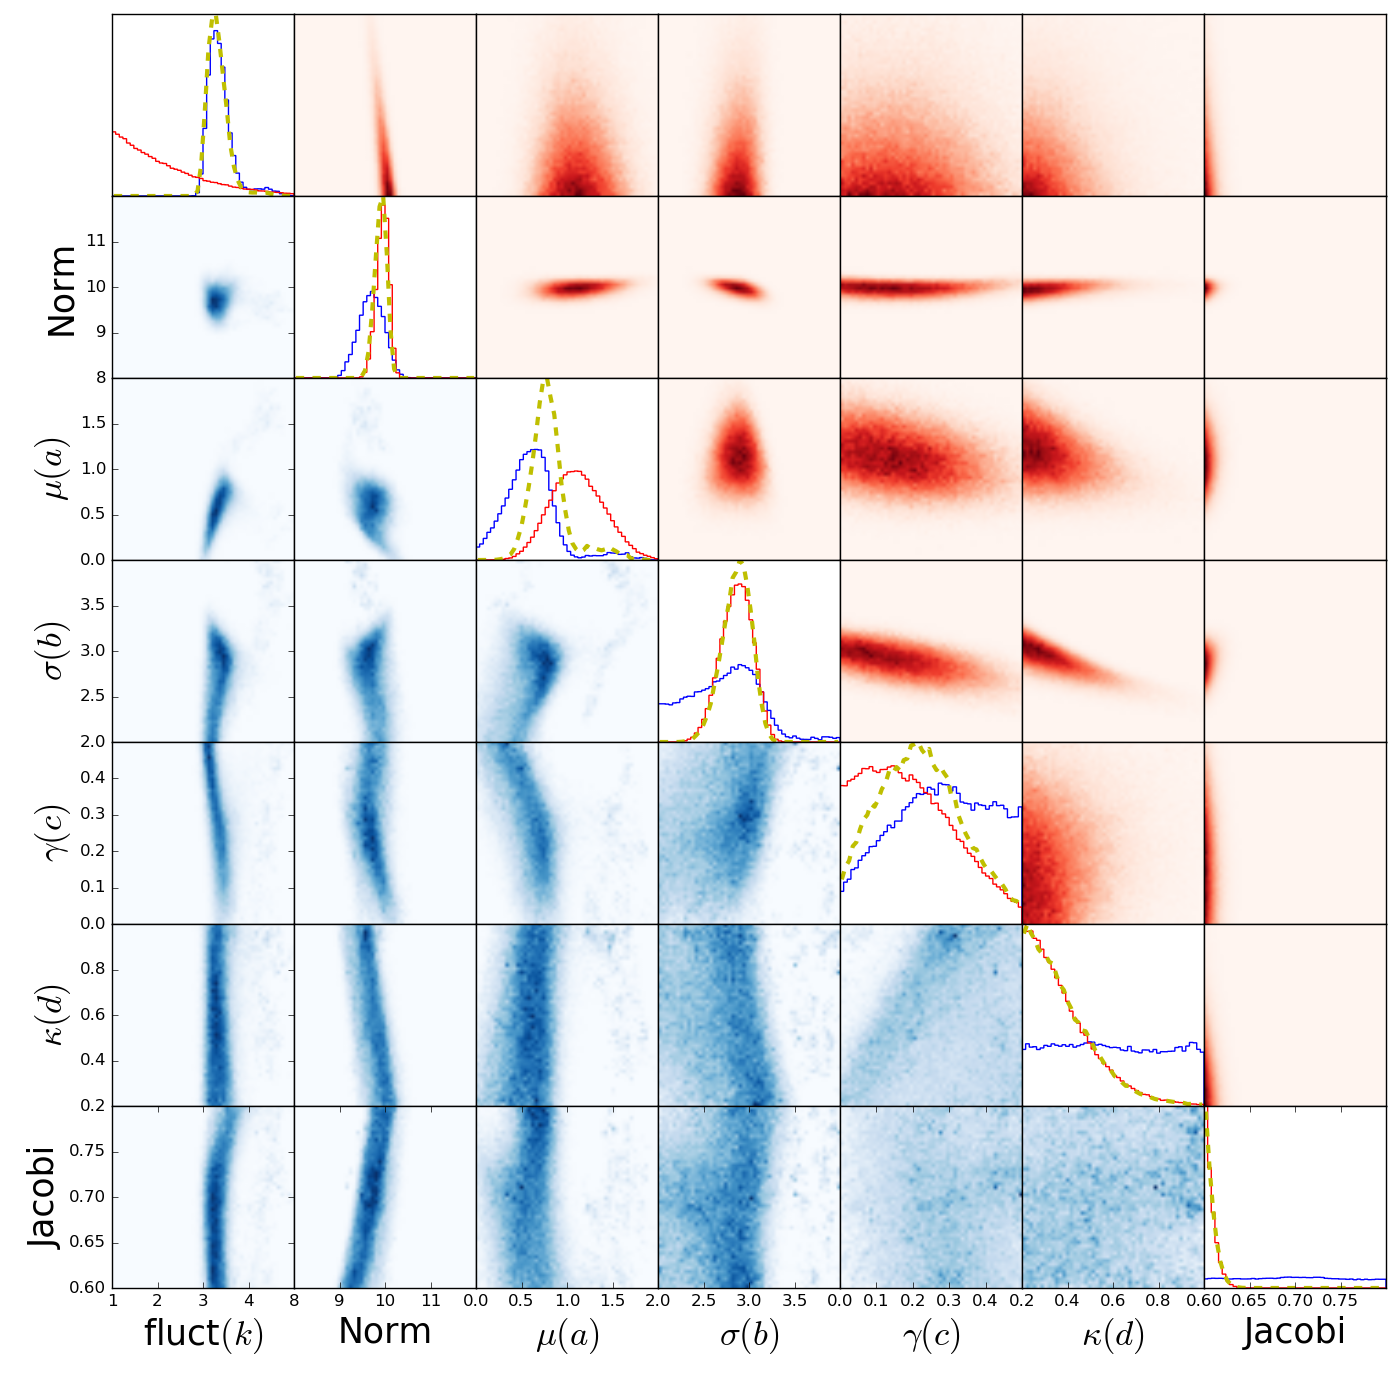
\includegraphics[width = \textwidth]{./pics/corner.png}
\end{center}
\end{figure}
\end{column}
\begin{column}{0.4\textwidth}
\begin{itemize}
\item Red: PbPb data.
\item Blue: pPb data.
\item Diagonal: $P(x_i)$. 
\item Off-diagonal: $P(x_i, x_j)$.
\end{itemize}
Observations:
\begin{itemize}
\item pPb sensitive to $k$.
\item PbPb sensitive to $\sigma$.
\item $\gamma, \mu$ correlation. 
\item Favours $\mu = 1$, small $\gamma$,
\begin{eqnarray}
\mu \sim \frac{1}{2}\ln(\frac{T_A}{T_B}).
\end{eqnarray}
\end{itemize}
\end{column}
\end{columns}
\end{frame}

\begin{frame}{Marginalized posterior distribution of model parameters}
\begin{itemize}
\item Compare TRENTo 3d initial condition with charged particle pseudo-rapidity distribution.
\item Suggest a slightly tilted longitudinal entropy deposition with its mean around the CoM rapidity of incoming participant densities.
\begin{eqnarray}
\mu(x_\perp) \sim \frac{1}{2}\ln\left(\frac{T_A(x_\perp)}{T_B(x_\perp)}\right).
\end{eqnarray}
\end{itemize}
\end{frame}

\begin{frame}{Effect of hydrodynamic evolution and re-scattering}
\begin{itemize}
\item Parameter sets around the maximum of posterior distribution \\ $\rightarrow$ perform full-time evolution.
\item Pseudo-critical temperature of EoS, $T_c = 0.154$ GeV.
\item Switching temperature of particularization, $T_{\textrm{sw}} = 0.148$ GeV.
\item Transport coefficients $\zeta/s = 0$, $\eta/s(T)$.
\begin{center}
\begin{figure}
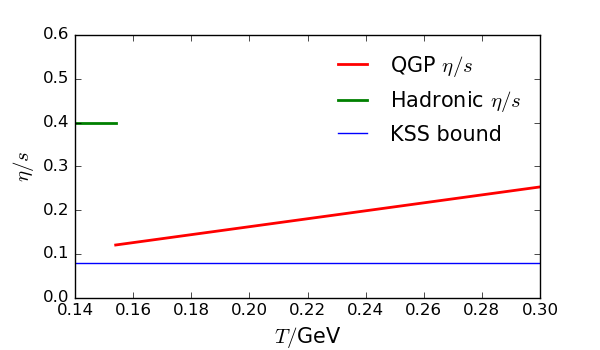
\includegraphics[width=0.6\textwidth]{./pics/trans_coeff.png}
\end{figure}
\end{center}
\end{itemize}
\end{frame}

\begin{frame}{Charged particle distribution}
\begin{itemize}
\item The general agreement of $\mathrm{d}N_{ch}/\mathrm{d}\eta$ with experiment is robust against evolution.
\item Validate the use of $\mathrm{d}N_{ch}\mathrm{d}\eta$ for model-to-data comparison for initial condition.
\end{itemize}
\begin{figure}
\begin{center}
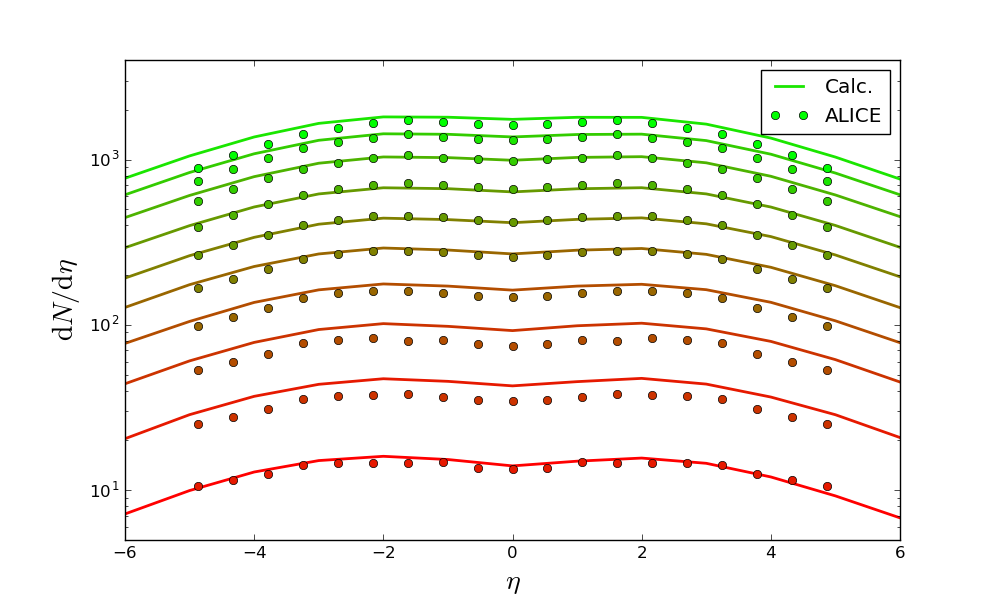
\includegraphics[width = 0.5\textwidth]{./pics/RUN-1-PbPb-dNdy-eta.png}
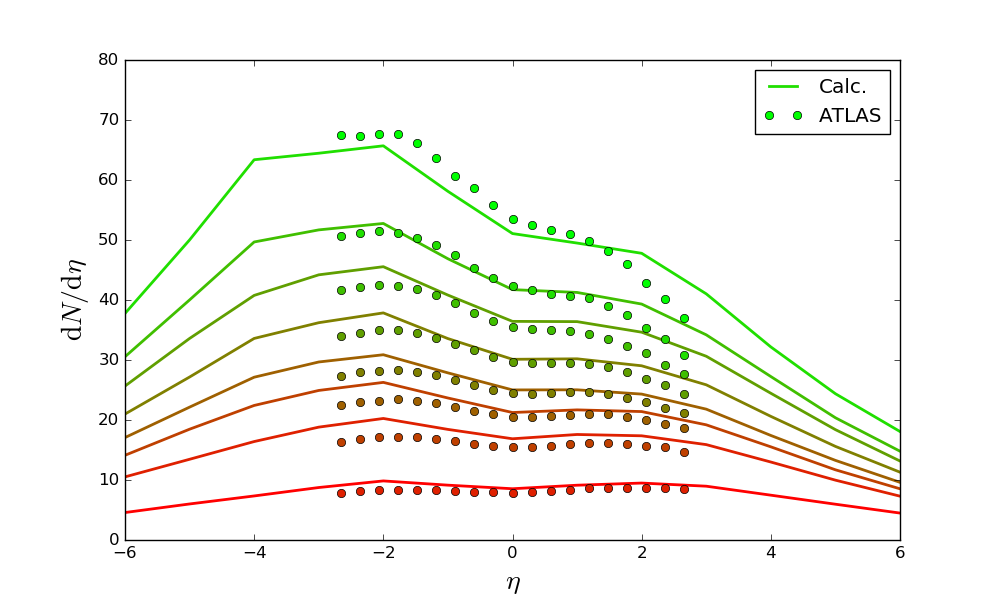
\includegraphics[width = 0.5\textwidth]{./pics/RUN-1-pPb-dNdy-eta.png}
\end{center}
\end{figure}
\end{frame}

\begin{frame}{Summary and outlook}
\begin{itemize}
\item Relativistic heavy-ion collision produces quark-gluon plasma (QGP).
\item QGP properties are inferred by model-to-data comparison.
\item Interest of rapidity dependent observables and small systems necessitates a rapidity dependent initial condition.
\item Extend TRENTo initial condition from 2d to 3d using a general formula.
\item Model-to-data comparison suggests a longitudinal distribution around the CoM rapidity.
\item Enlarged data set in future model-to-data comparison $\rightarrow$ improved knowledge on both IC and QGP properties.
\end{itemize}
\end{frame}
%----------------------------------------------------------------

%--------------------------Back up-------------------------------
\begin{frame}[noframenumbering]{Back up: Flow observables from 3d IC + time evolution}
\begin{figure}
\begin{center}
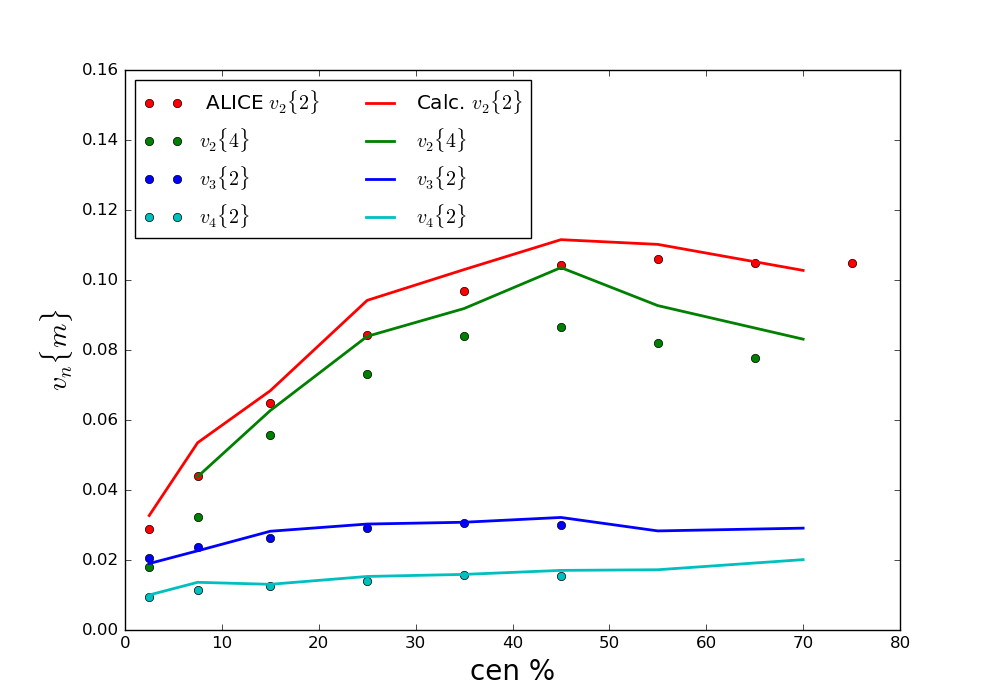
\includegraphics[width = 0.4\textwidth]{./pics/new-PbPb-vnm-p1.png}
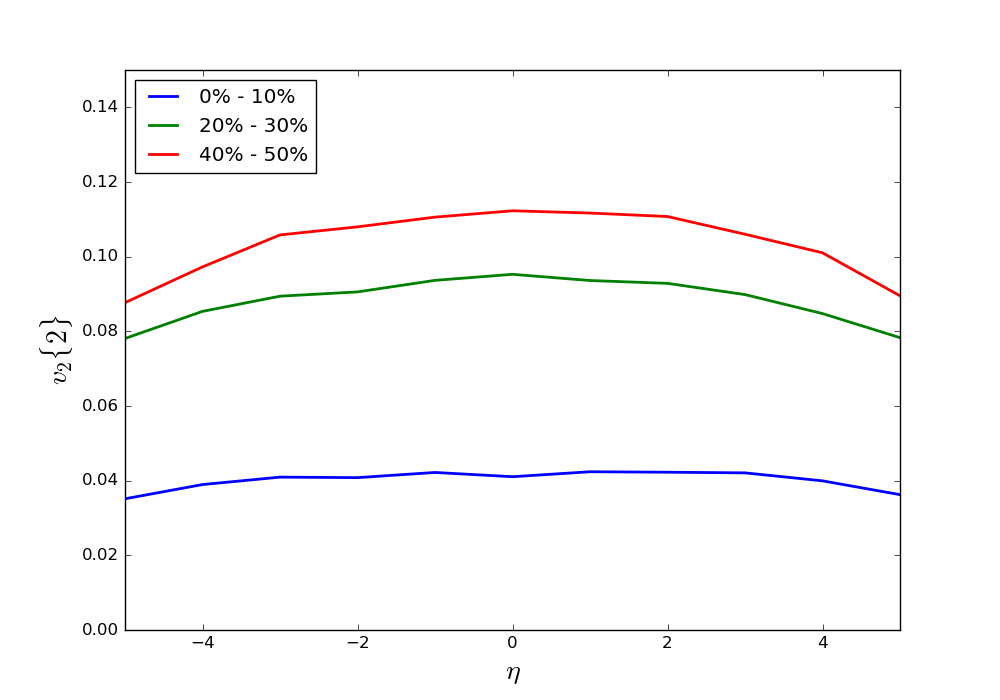
\includegraphics[width = 0.4\textwidth]{./pics/new-PbPb-vnm-eta-p1.png}\\
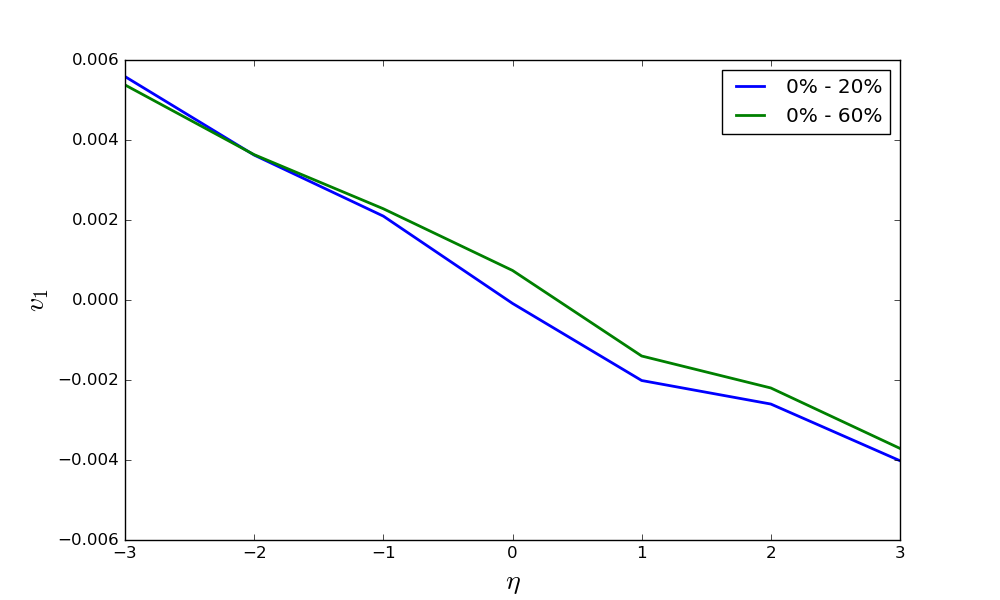
\includegraphics[width = 0.4\textwidth]{./pics/RUN-1-PbPb-v1-eta.png}
\end{center}
\end{figure}
\end{frame}

\begin{frame}[noframenumbering]{Back up: higher order flow}
\begin{itemize}
\item Fluctuation of initial geometry of the collision leads to higher order anisotropic flows.
\end{itemize}
\begin{center}
\begin{figure}
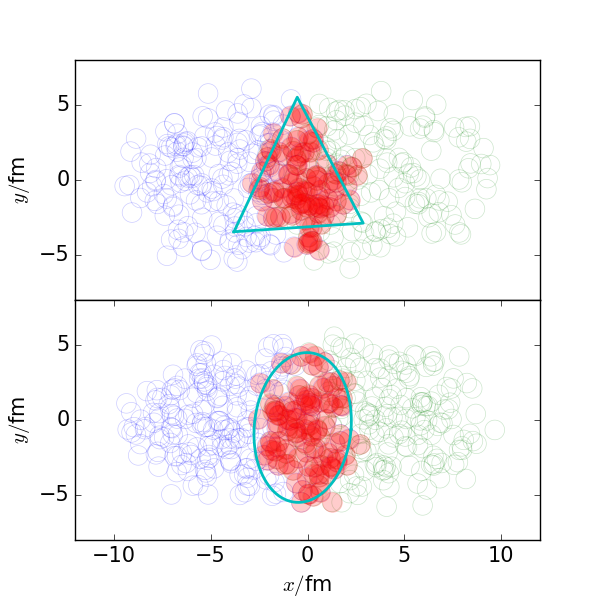
\includegraphics[width = 0.5\textwidth]{./pics/nuclei.png}
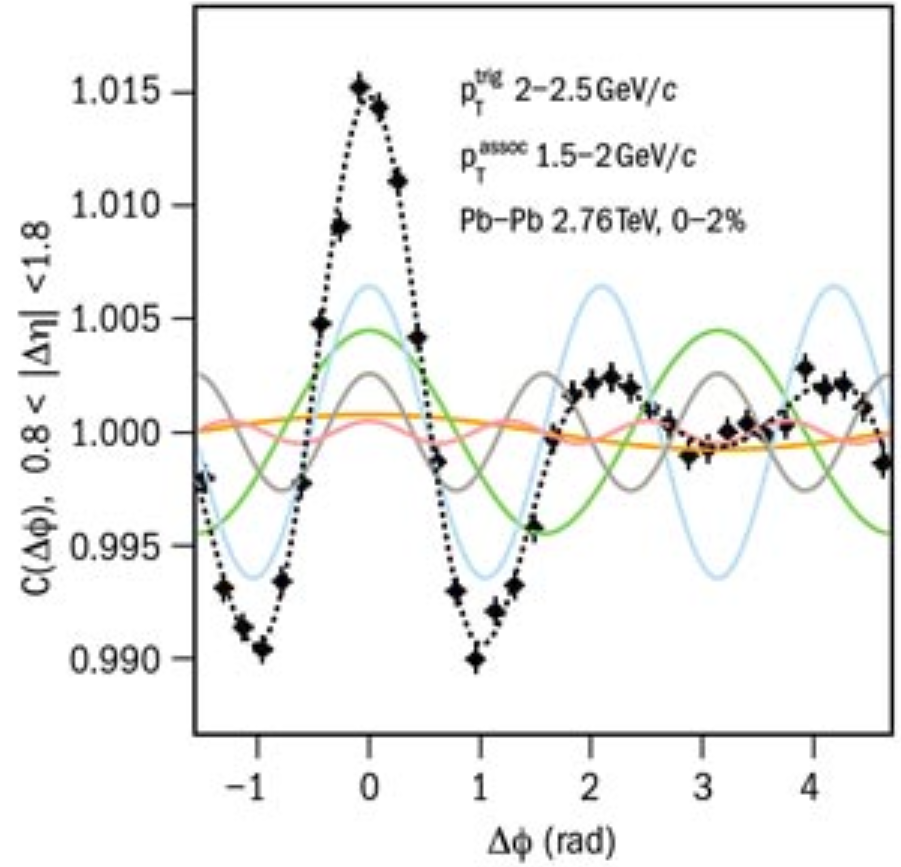
\includegraphics[width = 0.45\textwidth]{./pics/corr_ALICE.png}
\end{figure}
\end{center}
\end{frame}

\begin{frame}[noframenumbering]{Back up: $\eta/s$ for different fluid}
\begin{itemize}
\item Extract $\eta/s$ by comparing model calculation with experimental data.
\item Extremely low $\eta/s \sim 0.08 - 0.20$, close to quantum lower bound of $\eta/s = \frac{1}{4\pi}$ $\rightarrow$ almost perfect liquid.
\item \color{red}Large uncertainty from initial conditions.
\end{itemize}
\begin{figure}
\begin{center}
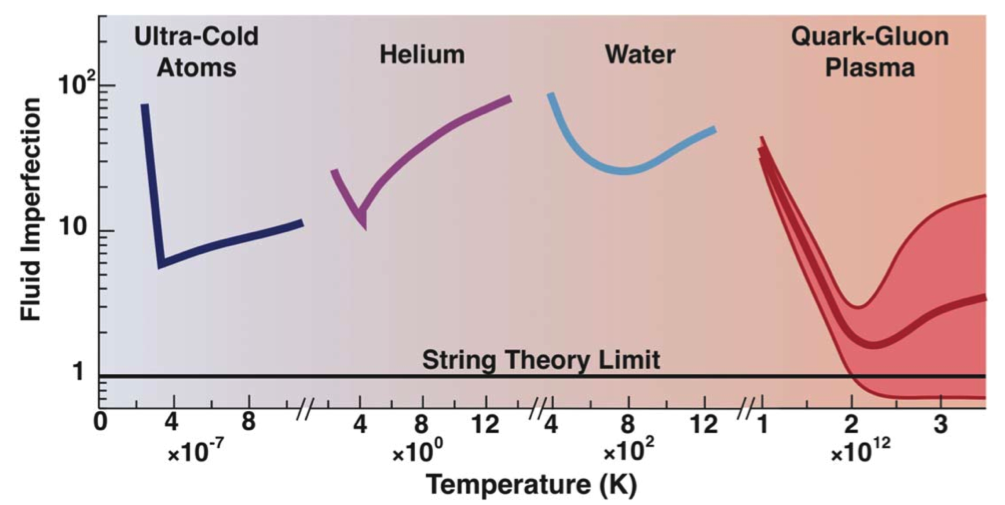
\includegraphics[width=0.6\textwidth]{pics/eta_s.png} 
\end{center} 	
\end{figure}
\end{frame}

\begin{frame}[noframenumbering]{Back up: isothermal hyper-surface}
\begin{columns}[onlytextwidth]
  \begin{column}{0.2\textwidth}
    \begin{figure}
   	\begin{center}
   	\includegraphics[width=\textwidth]{pics/new230.png}
	\end{center} 	
  	\end{figure}
  \end{column}
  \begin{column}{0.8\textwidth}
  \begin{itemize}
  	\item The expanding system becomes dilute and hydrodynamics ceases to apply.
  	\item Particlize energy density to hadrons.
  \end{itemize}
  \end{column}
\end{columns}

\begin{columns}[onlytextwidth]
  \begin{column}{0.6\textwidth}
  \begin{itemize}
	\item Particles are sampled from a constant temperature hyper-surface:
	\begin{eqnarray}
	E\frac{\mathrm{d}N_i}{\mathrm{d}^3p} = \int_\Sigma f_i(x, p)p^\mu\mathrm{d}^3\sigma_\mu.
	\end{eqnarray}
	\item $f_i$ is the distribution function of particle type ``$i$" and $\mathrm{d}\sigma_\mu$ is the surface element.
  \end{itemize}
  \end{column}
  \begin{column}{0.4\textwidth}
    \begin{figure}
   	\begin{center}
   	\includegraphics[width=\textwidth]{pics/freeze.png}
	\end{center} 	
  	\end{figure}
  \end{column}
\end{columns}
\end{frame}


\begin{frame}[noframenumbering]{Back up: hadronic re-scattering $\rightarrow$ calculation meets experiment}
\begin{columns}
 \begin{column}{0.2\textwidth}
    \begin{figure}
   	\begin{center}
   	\includegraphics[width=\textwidth]{pics/new300.png}
	\end{center} 	
  	\end{figure}
  \end{column}
  \begin{column}{0.8\textwidth}
  \begin{itemize}
  	\item System is still dense to allow hadronic scattering.
	\item Solving Boltzmann transport equation, 
		\begin{eqnarray}
		\frac{\mathrm{d}}{\mathrm{d}t}f_i(x, p) = C_i(x, p).
		\end{eqnarray}
		 RHS: gain and loss of particles due to collisions.
  \end{itemize}
  \end{column}
\end{columns}
\begin{columns}
 \begin{column}{0.6\textwidth}
  \begin{itemize}
  	\item Implementation: Ultra-relativistic Quantum Molecular Dynamics (UrQMD). 
  	\item Extract experimental observables from hadrons final states.
  \end{itemize}
  \end{column}
  \begin{column}{0.4\textwidth}
      \begin{figure}
   	\begin{center}
   	\includegraphics[width=\textwidth]{pics/CMS.png}
	\end{center} 	
  	\end{figure}
  \end{column}
\end{columns}
\end{frame}

\begin{frame}[noframenumbering]{Back up: centrality class and collision geometry}
\begin{itemize}
\item Interested in initial spatial anisotropy (eccentricity).
\item Experimental no control over initial eccentricity.
\end{itemize}
\begin{center}
\begin{tabular}{cccc}
\hline 
Impact parameter & Overlap & Multiplicity & Eccentricity \\
\hline
Large & Small & \color{red}Small & \color{red}Large \\  
Small & Large & \color{red}Large & \color{red}Small \\ 
\hline 
\end{tabular} 
\end{center}
\begin{figure}
\begin{center}
\includegraphics[width = 0.9\textwidth]{./pics/centrality.png}
\end{center}
\end{figure}
\end{frame}

\begin{frame}[noframenumbering]{Back up: more on flow observables}
\begin{columns}
 \begin{column}{0.5\textwidth}
    \begin{figure}
   	\begin{center}
   	\includegraphics[width=0.8\textwidth]{pics/Gale-1.png}
	\end{center} 	
  	\end{figure}
  \end{column}
  \begin{column}{0.5\textwidth}
  	\begin{figure}
   	\begin{center}
   	\includegraphics[width=0.8\textwidth]{pics/Gale-2.png}
	\end{center} 	
  	\end{figure}
  \end{column}
\end{columns}
\end{frame}


\begin{frame}[noframenumbering]{Back up: uncertainty in IC affects transport properties extraction}
\begin{itemize}
\item Varying $p$ $\rightarrow$ continuously interpolates existing models.
\end{itemize}
\begin{center}
\begin{figure}
\includegraphics[width = 0.45\textwidth]{./pics/interp.png}
\includegraphics[width = 0.55\textwidth]{./pics/trento-vs-glasma.pdf}
\end{figure}
\end{center}
\end{frame}

\begin{frame}[noframenumbering]{Back up: more rapidity dependent observables}
\begin{itemize}
\item Directed flow: deflection of produced matter away from beam axis.
\item Directed flow could be sensitive to EoS and IC.
\end{itemize}
\begin{center}
\begin{figure}
\includegraphics[width=0.4\textwidth]{./pics/Pitor-0.png}
\includegraphics[width=0.4\textwidth]{./pics/Pitor-1.png}
\end{figure}
\end{center}
\end{frame}

\begin{frame}[noframenumbering]{Back up: regulating cumulants generating function}
\begin{itemize}
\item The reconstructed function may not be well-behaved.
\item To regulate (\ref{naive_fourier}) and result in well behaved function,
\begin{eqnarray}
 \gamma \rightarrow \gamma\exp\left(-\sigma^2k^2/2\right), \kappa \rightarrow \kappa\exp\left(-\sigma^2k^2/2\right). 
\end{eqnarray}
\end{itemize}
\begin{center}
\begin{figure}
\includegraphics[width=0.75\textwidth]{pics/regulate.png}
\end{figure}
\end{center}
\end{frame}

\begin{frame}{Back up: Bayes' theorem}
\begin{itemize}
\item Posterior probability distribution of parameters by Bayes' theorem.
\begin{eqnarray}
P(x^* | \{\mathbf{x}_i, y_i\}, y_{\textrm{exp}} )
 \propto P(y_{\textrm{exp}}|\{\mathbf{x}_i, y_i\}, x^*) P(x^*).
\end{eqnarray}
Prior: $P(x^*)$, posterior $P(x^* | \{\mathbf{x}_i, y_i\}, y_{\textrm{exp}} )$.
\item Study this high posterior dimensional distribution function by Markov-chain Monte-Carlo procedure.
\end{itemize}
\end{frame}

\begin{frame}[noframenumbering]{Back up: high dimensional data reduction}
\begin{itemize}
\item Model outputs are high dimensional vector.
\item Redundant and impractical to emulate each component.
\item Principal Component Analysis (PCA): reduce high dimensional output to a few principal components that covers most of the data variance.
\item Model output is recovered by transforming back the truncated principal components.
\end{itemize}
\end{frame}

\begin{frame}[noframenumbering]{Back up: model-to-data comparison details}
\begin{itemize}
\item A 100 sets of parameters are sampled within reasonable ranges.
\item 1000 events are generated for PbPb and pPb systems.
\item $\mathrm{d}S/\mathrm{d}\eta_s$ calculated for each centrality case; compared to $\mathrm{d}N_{\textrm{ch}}/\mathrm{d}\eta$
\item Perform PCA on $\mathrm{d}S/\mathrm{d}\eta_s$, and take the first 5 principal components.
\item Generate $10^6$ samples from posterior distribution usuing MCMC.
\begin{figure}
\begin{center}
\includegraphics[width = 0.6\textwidth]{./pics/weight.png}
\end{center}
\end{figure}
\end{itemize}
\end{frame}
%----------------------------------------------------------------
\end{document}